% Options for packages loaded elsewhere
\PassOptionsToPackage{unicode}{hyperref}
\PassOptionsToPackage{hyphens}{url}
%
\documentclass[
]{book}
\usepackage{lmodern}
\usepackage{amssymb,amsmath}
\usepackage{ifxetex,ifluatex}
\ifnum 0\ifxetex 1\fi\ifluatex 1\fi=0 % if pdftex
  \usepackage[T1]{fontenc}
  \usepackage[utf8]{inputenc}
  \usepackage{textcomp} % provide euro and other symbols
\else % if luatex or xetex
  \usepackage{unicode-math}
  \defaultfontfeatures{Scale=MatchLowercase}
  \defaultfontfeatures[\rmfamily]{Ligatures=TeX,Scale=1}
\fi
% Use upquote if available, for straight quotes in verbatim environments
\IfFileExists{upquote.sty}{\usepackage{upquote}}{}
\IfFileExists{microtype.sty}{% use microtype if available
  \usepackage[]{microtype}
  \UseMicrotypeSet[protrusion]{basicmath} % disable protrusion for tt fonts
}{}
\makeatletter
\@ifundefined{KOMAClassName}{% if non-KOMA class
  \IfFileExists{parskip.sty}{%
    \usepackage{parskip}
  }{% else
    \setlength{\parindent}{0pt}
    \setlength{\parskip}{6pt plus 2pt minus 1pt}}
}{% if KOMA class
  \KOMAoptions{parskip=half}}
\makeatother
\usepackage{xcolor}
\IfFileExists{xurl.sty}{\usepackage{xurl}}{} % add URL line breaks if available
\IfFileExists{bookmark.sty}{\usepackage{bookmark}}{\usepackage{hyperref}}
\hypersetup{
  pdftitle={R en las Ciencias Agropecuarias},
  pdfauthor={Franklin Santos},
  hidelinks,
  pdfcreator={LaTeX via pandoc}}
\urlstyle{same} % disable monospaced font for URLs
\usepackage{color}
\usepackage{fancyvrb}
\newcommand{\VerbBar}{|}
\newcommand{\VERB}{\Verb[commandchars=\\\{\}]}
\DefineVerbatimEnvironment{Highlighting}{Verbatim}{commandchars=\\\{\}}
% Add ',fontsize=\small' for more characters per line
\usepackage{framed}
\definecolor{shadecolor}{RGB}{248,248,248}
\newenvironment{Shaded}{\begin{snugshade}}{\end{snugshade}}
\newcommand{\AlertTok}[1]{\textcolor[rgb]{0.94,0.16,0.16}{#1}}
\newcommand{\AnnotationTok}[1]{\textcolor[rgb]{0.56,0.35,0.01}{\textbf{\textit{#1}}}}
\newcommand{\AttributeTok}[1]{\textcolor[rgb]{0.77,0.63,0.00}{#1}}
\newcommand{\BaseNTok}[1]{\textcolor[rgb]{0.00,0.00,0.81}{#1}}
\newcommand{\BuiltInTok}[1]{#1}
\newcommand{\CharTok}[1]{\textcolor[rgb]{0.31,0.60,0.02}{#1}}
\newcommand{\CommentTok}[1]{\textcolor[rgb]{0.56,0.35,0.01}{\textit{#1}}}
\newcommand{\CommentVarTok}[1]{\textcolor[rgb]{0.56,0.35,0.01}{\textbf{\textit{#1}}}}
\newcommand{\ConstantTok}[1]{\textcolor[rgb]{0.00,0.00,0.00}{#1}}
\newcommand{\ControlFlowTok}[1]{\textcolor[rgb]{0.13,0.29,0.53}{\textbf{#1}}}
\newcommand{\DataTypeTok}[1]{\textcolor[rgb]{0.13,0.29,0.53}{#1}}
\newcommand{\DecValTok}[1]{\textcolor[rgb]{0.00,0.00,0.81}{#1}}
\newcommand{\DocumentationTok}[1]{\textcolor[rgb]{0.56,0.35,0.01}{\textbf{\textit{#1}}}}
\newcommand{\ErrorTok}[1]{\textcolor[rgb]{0.64,0.00,0.00}{\textbf{#1}}}
\newcommand{\ExtensionTok}[1]{#1}
\newcommand{\FloatTok}[1]{\textcolor[rgb]{0.00,0.00,0.81}{#1}}
\newcommand{\FunctionTok}[1]{\textcolor[rgb]{0.00,0.00,0.00}{#1}}
\newcommand{\ImportTok}[1]{#1}
\newcommand{\InformationTok}[1]{\textcolor[rgb]{0.56,0.35,0.01}{\textbf{\textit{#1}}}}
\newcommand{\KeywordTok}[1]{\textcolor[rgb]{0.13,0.29,0.53}{\textbf{#1}}}
\newcommand{\NormalTok}[1]{#1}
\newcommand{\OperatorTok}[1]{\textcolor[rgb]{0.81,0.36,0.00}{\textbf{#1}}}
\newcommand{\OtherTok}[1]{\textcolor[rgb]{0.56,0.35,0.01}{#1}}
\newcommand{\PreprocessorTok}[1]{\textcolor[rgb]{0.56,0.35,0.01}{\textit{#1}}}
\newcommand{\RegionMarkerTok}[1]{#1}
\newcommand{\SpecialCharTok}[1]{\textcolor[rgb]{0.00,0.00,0.00}{#1}}
\newcommand{\SpecialStringTok}[1]{\textcolor[rgb]{0.31,0.60,0.02}{#1}}
\newcommand{\StringTok}[1]{\textcolor[rgb]{0.31,0.60,0.02}{#1}}
\newcommand{\VariableTok}[1]{\textcolor[rgb]{0.00,0.00,0.00}{#1}}
\newcommand{\VerbatimStringTok}[1]{\textcolor[rgb]{0.31,0.60,0.02}{#1}}
\newcommand{\WarningTok}[1]{\textcolor[rgb]{0.56,0.35,0.01}{\textbf{\textit{#1}}}}
\usepackage{longtable,booktabs}
% Correct order of tables after \paragraph or \subparagraph
\usepackage{etoolbox}
\makeatletter
\patchcmd\longtable{\par}{\if@noskipsec\mbox{}\fi\par}{}{}
\makeatother
% Allow footnotes in longtable head/foot
\IfFileExists{footnotehyper.sty}{\usepackage{footnotehyper}}{\usepackage{footnote}}
\makesavenoteenv{longtable}
\usepackage{graphicx,grffile}
\makeatletter
\def\maxwidth{\ifdim\Gin@nat@width>\linewidth\linewidth\else\Gin@nat@width\fi}
\def\maxheight{\ifdim\Gin@nat@height>\textheight\textheight\else\Gin@nat@height\fi}
\makeatother
% Scale images if necessary, so that they will not overflow the page
% margins by default, and it is still possible to overwrite the defaults
% using explicit options in \includegraphics[width, height, ...]{}
\setkeys{Gin}{width=\maxwidth,height=\maxheight,keepaspectratio}
% Set default figure placement to htbp
\makeatletter
\def\fps@figure{htbp}
\makeatother
\setlength{\emergencystretch}{3em} % prevent overfull lines
\providecommand{\tightlist}{%
  \setlength{\itemsep}{0pt}\setlength{\parskip}{0pt}}
\setcounter{secnumdepth}{5}
\usepackage{booktabs}
\usepackage[]{natbib}
\bibliographystyle{apalike}

\title{R en las Ciencias Agropecuarias}
\author{Franklin Santos}
\date{2020-11-23}

\begin{document}
\maketitle

{
\setcounter{tocdepth}{1}
\tableofcontents
}
\hypertarget{bienvenido}{%
\chapter*{Bienvenido}\label{bienvenido}}
\addcontentsline{toc}{chapter}{Bienvenido}

Bienvenido a \textbf{R aplicada en las Ciencias Agropecuarias}. El contenido del libro presenta ejemplos de análisis exploratorio de datos, estadística inferencial y modelos de regresión. Generalmente, se expone las metodologías mas usuales en un reporte de trabajos de investigación y/o tesis.

Este libro es para aquellos que tienen poca o ninguna experiencia previa en programación en R o cualquier otro lenguaje de programación. Su objetivo es desarrollar los conceptos básicos y enseñarle las capacidades de R. Con la lectura y práctica, habrá adquirido una nueva habilidad valiosa para explorar conjuntos de datos y crear visualizaciones impresionantes.

\hypertarget{prerequisites}{%
\section{Prerequisites}\label{prerequisites}}

This is a \emph{sample} book written in \textbf{Markdown}. You can use anything that Pandoc's Markdown supports, e.g., a math equation \(a^2 + b^2 = c^2\).

The \textbf{bookdown} package can be installed from CRAN or Github:

\begin{Shaded}
\begin{Highlighting}[]
\KeywordTok{install.packages}\NormalTok{(}\StringTok{"bookdown"}\NormalTok{)}
\CommentTok{# or the development version}
\CommentTok{# devtools::install_github("rstudio/bookdown")}
\end{Highlighting}
\end{Shaded}

Remember each Rmd file contains one and only one chapter, and a chapter is defined by the first-level heading \texttt{\#}.

To compile this example to PDF, you need XeLaTeX. You are recommended to install TinyTeX (which includes XeLaTeX): \url{https://yihui.org/tinytex/}.

\hypertarget{intro}{%
\chapter{R básico}\label{intro}}

R es muy popular e increíblemente útil para las personas que trabajan como científicos de datos o en empresas. Pero también puede usar R para cosas más simples, como crear un gráfico agradable o hacer un cálculo rápido. Comenzar a utilizar R es bastante sencillo.

\hypertarget{introducciuxf3n-a-r}{%
\section{Introducción a R}\label{introducciuxf3n-a-r}}

\begin{quote}
El lenguaje informático estadístico más potente del planeta.
-- Norman Nie, fundador de SPSS
\end{quote}

R es un lenguaje de programación y un ambiente para trabajar con datos. Es muy utilizado por estadísticos y científicos de datos por su sintaxis de código expresivo, abundantes paquetes y herramientas externas y funciona en todos los sistemas operativos principales.

Es la navaja suiza para el análisis de datos y la computación estadística (¡y también puedes hacer algunos gráficos bonitos!). El lenguaje R se puede ampliar fácilmente con paquetes escritos por una gran y creciente comunidad de desarrolladores de todo el mundo. Puede encontrarlo prácticamente en cualquier lugar: lo utilizan instituciones académicas, empresas emergentes, corporaciones internacionales y muchos más.

\hypertarget{por-quuxe9-usar-r}{%
\subsection{¿Por qué usar R?}\label{por-quuxe9-usar-r}}

R es un lenguaje popular para resolver problemas de análisis de datos y también lo usan personas que tradicionalmente no se consideran programadores. Al crear gráficos y visualizaciones con R, descubrirá que tiene muchas más posibilidades creativas que las aplicaciones gráficas, como Excel.

Estas son algunas de las \textbf{características} por las que R es más famoso:

\textbf{Visualización}: Crear gráficos y visualizaciones hermosos, es una de sus mayores fortalezas. El lenguaje central ya proporciona un amplio conjunto de herramientas utilizadas para trazar gráficos y para todo tipo de gráficos. El cielo es el límite.

\textbf{Reproducibilidad}: a diferencia del software de hoja de cálculo, el código R no está acoplado a conjuntos de datos específicos y puede reutilizarse fácilmente en diferentes proyectos, incluso cuando excede más de 1 millón de filas. Cree fácilmente informes reutilizables y genere automáticamente nuevas versiones a medida que cambien los datos.

\textbf{Modelamiento avanzado}: R proporciona la base de código más grande y poderosa para el análisis de datos en el mundo. La riqueza y profundidad de los modelos estadísticos disponibles no tiene paralelo y crece día a día, gracias a la gran comunidad de desarrolladores y colaboradores de paquetes de código abierto.

\textbf{Automatización}: el código R también se puede utilizar para automatizar informes o para realizar transformación de datos y cálculos de modelos. También se puede integrar en flujos de trabajo de producción automatizados, ambientes informáticos en la nube y sistemas de bases de datos modernos.

\hypertarget{r-en-buena-compauxf1uxeda}{%
\subsection{R en buena compañía}\label{r-en-buena-compauxf1uxeda}}

R es el estándar de facto para la computación estadística en instituciones académicas y empresas de todo el mundo. Su gran soporte para la programación alfabetizada (código que se puede combinar con texto legible por humanos) permite a los investigadores y científicos de datos crear informes listos para publicación que son fáciles de reproducir para los revisores.

El lenguaje ha tenido una amplia adopción en varias industrias; vea algunos ejemplos a continuación:

\textbf{Tecnologías de la información}

\begin{itemize}
\item
  Microsoft: \href{https://mran.microsoft.com/open}{Microsoft R Open}, \href{https://www.microsoft.com/en-us/research/publication/trueskilltm-a-bayesian-skill-rating-system}{TrueSkill(TM)}, más \href{https://blog.revolutionanalytics.com/2018/02/what-does-microsoft-do-with-r.html}{aquí}
\item
  Google: \href{https://research.google/pubs/pub43342/}{R para investigación de mercado y análisis}, \href{https://static.googleusercontent.com/media/www.google.com/fr//googleblogs/pdfs/google_predicting_the_present.pdf}{prediciendo el presente con Google Trends}
\item
  Facebook: \href{https://www.facebook.com/notes/facebook-engineering/visualizing-friendships/469716398919}{Visualizando amistades}, \href{https://www.facebook.com/notes/facebook-data-science/the-formation-of-love/10152064609253859}{La formación del amor}, Paquete \href{https://facebook.github.io/prophet}{Prophet} para pronósticos de series de tiempo.
\item
  Otros (con enlaces a proyectos): \href{https://peerj.com/preprints/3182.pdf}{AirBnB}, \href{https://capetown2017.satrdays.org/talks/satRday-2017-van-heerden.pdf}{Uber}, \href{https://www.oracle.com/database/technologies/datawarehouse-bigdata/oml4r.html}{Oracle}, IBM, Twitter.
\end{itemize}

\textbf{Farmacias}: Merck, Genentech (Roche), Novartis, Pfizer
\textbf{Periódicos}: The Economist, The New York Times, Financial Times

\textbf{Finanzas}

\begin{itemize}
\item
  Bancos: Bank of America, J.P.Morgan, Goldman Sachs, Credit Suisse, UBS, Deutsche Bank
\item
  Seguros: Lloyd's, Allianz
\end{itemize}

\hypertarget{bloques-de-construcciuxf3n}{%
\section{Bloques de construcción}\label{bloques-de-construcciuxf3n}}

El lenguaje R consta de tres bloques fundamentales de construcción necesarios para realizar sus primeros pasos en el ambiente R:

\begin{itemize}
\tightlist
\item
  Objeto: todo lo que existe es un objeto
\item
  Función: todo lo que sucede es una llamada a función
\item
  Interfaz: R se basa en interfaces para muchos algoritmos
\end{itemize}

Los \textbf{objetos} más importantes en R son \textbf{vectores}. Forman la base de (casi) todas las estructuras de datos de R. La mayor parte del poder y la expresividad de R se deriva del hecho de que es un lenguaje orientado a vectores. Las \textbf{funciones} y los operadores pueden definirse fácilmente y trabajar directamente en vectores para calcular resultados.

La mayor fortaleza de R es su flexibilidad para integrar fácilmente nuevos algoritmos y construir \textbf{interfaces} a su alrededor. El sistema de paquetes R permite a los colaboradores integrar muchos modelos y bibliotecas externas de código abierto. Su repositorio principal de paquetes llamado ``\textbf{CRAN}'' aloja estos paquetes y permite a los usuarios instalarlos y cargarlos fácilmente en sus ambientes.

\hypertarget{combinar-valores-en-un-vector}{%
\section{Combinar valores en un vector}\label{combinar-valores-en-un-vector}}

R siempre crea listas de valores, incluso cuando solo hay un valor en una lista. Estas listas se denominan vectores y facilitan mucho el trabajo con datos.

\begin{itemize}
\tightlist
\item
  Todo es un vector
\item
  Conozca los diferentes tipos de datos en R
\item
  Aprenda a crear vectores
\item
  Utilice el operador \texttt{:} para crear secuencias numéricas
\item
  Utilice la función de concatenar \texttt{c()} para crear vectores de diferentes tipos de datos
\end{itemize}

\begin{Shaded}
\begin{Highlighting}[]
\DecValTok{1}\OperatorTok{:}\DecValTok{100}
\KeywordTok{c}\NormalTok{(}\DecValTok{1}\NormalTok{, }\DecValTok{2}\NormalTok{, }\DecValTok{3}\NormalTok{, }\DecValTok{4}\NormalTok{)}
\KeywordTok{c}\NormalTok{(}\StringTok{"abc"}\NormalTok{, }\StringTok{"def"}\NormalTok{, }\StringTok{"ghi"}\NormalTok{)}
\KeywordTok{c}\NormalTok{(}\OtherTok{TRUE}\NormalTok{, }\OtherTok{FALSE}\NormalTok{, }\OtherTok{TRUE}\NormalTok{)}
\end{Highlighting}
\end{Shaded}

\hypertarget{introducciuxf3n-a-los-vectores}{%
\subsection{Introducción a los vectores}\label{introducciuxf3n-a-los-vectores}}

Un vector es una colección de elementos del mismo tipo y la estructura de datos más básica en R. Por ejemplo, un vector podría contener los cuatro números \texttt{1}, \texttt{3}, \texttt{2} y \texttt{5}. Otro vector podría formarse con las tres cadenas de texto \texttt{"Bienvenido"},\texttt{"Hi"} y \texttt{"Hola"}. Estos diferentes tipos de valores (números, texto) se denominan \emph{tipos de datos}.

Un valor único también se trata como un vector, un vector con un solo elemento. Como veremos a lo largo del curso, este concepto hace que R sea muy especial. Podemos manipular los vectores y sus valores a través de muchas operaciones proporcionadas por R.

Una ventaja clave de los vectores es que podemos aplicar una operación (por ejemplo, una multiplicación) a todos sus valores a la vez en lugar de pasar por cada elemento individualmente. Esto se llama \emph{vectorización}.

\hypertarget{tipos-de-vectores}{%
\subsection{Tipos de vectores}\label{tipos-de-vectores}}

Los vectores solo pueden contener elementos del mismo \emph{tipo de datos}. En este libro trabajaremos con los siguientes tres tipos de datos principales:

Los valores \textbf{numéricos} son números. Aunque pueden dividirse aún más en números enteros (enteros) y números con decimales (dobles), R convierte automáticamente entre estos subtipos si es necesario. Por lo tanto, colectivamente nos referiremos a ellos como valores \texttt{numéricos}.

Los valores de \textbf{caracteres} contienen contenido textual. Estos pueden ser letras, símbolos, espacios y números también. Deben estar entre comillas: comillas simples \texttt{\textquotesingle{}\_\_\_\textquotesingle{}} o comillas dobles \texttt{"\_\_\_"}.

Los valores \textbf{lógicos} pueden ser \texttt{TRUE} o \texttt{FALSE}. A menudo también se les conoce como valores \emph{booleanos} o \emph{binarios}. Debido a que un valor \texttt{lógico} solo puede ser \texttt{TRUE} o \texttt{FALSE}, se usan con mayor frecuencia para responder preguntas simples como ``¿Es 1 mayor que 2?'' o ``¿Son más de las 3 en punto?''. Este tipo de preguntas solo necesitan respuestas como ``Sí'' (\texttt{TRUE}) o ``No'' (\texttt{FALSE}). Es importante destacar que en R los valores \texttt{lógicos} distinguen entre mayúsculas y minúsculas, lo que significa que deben escribirse con mayúsculas.

\hypertarget{creando-una-secuencia-de-nuxfameros}{%
\subsection{Creando una secuencia de números}\label{creando-una-secuencia-de-nuxfameros}}

En R, incluso un solo valor se considera un vector. Crear un vector de un elemento es tan simple como escribir su valor:

\texttt{Código\ de\ entrada:}

\begin{Shaded}
\begin{Highlighting}[]
\DecValTok{4}
\end{Highlighting}
\end{Shaded}

\texttt{Resultado:}

\begin{verbatim}
## [1] 4
\end{verbatim}

Para crear una secuencia de valores numéricos, podemos usar el operador \texttt{:} que toma dos números y genera un vector de todos los números enteros en ese rango:

\texttt{Código\ de\ entrada:}

\begin{Shaded}
\begin{Highlighting}[]
\DecValTok{2}\OperatorTok{:}\DecValTok{11}
\end{Highlighting}
\end{Shaded}

\texttt{Resultado:}

\begin{verbatim}
##  [1]  2  3  4  5  6  7  8  9 10 11
\end{verbatim}

El operador \texttt{:} crea un vector desde el número en el lado izquierdo hasta el número en el lado derecho. Por lo tanto, el orden de los números es importante. Si definimos el ejemplo anterior al revés, obtenemos un vector de números descendentes, en lugar de ascendentes:

\texttt{Código\ de\ entrada:}

\begin{Shaded}
\begin{Highlighting}[]
\DecValTok{11}\OperatorTok{:}\DecValTok{2}
\end{Highlighting}
\end{Shaded}

\texttt{Resultado:}

\begin{verbatim}
##  [1] 11 10  9  8  7  6  5  4  3  2
\end{verbatim}

El operador \texttt{:} es útil cuando necesitamos un vector de cada número entero en un rango dado. Sin embargo, si necesitamos un vector donde los números no sean lineales, necesitamos algo diferente.

\hypertarget{concatenando-valores-numuxe9ricos-a-un-vector}{%
\subsection{Concatenando valores numéricos a un vector}\label{concatenando-valores-numuxe9ricos-a-un-vector}}

Podemos combinar múltiples números en un solo vector usando la función concatenar \texttt{c()} que une elementos entre las llaves redondas en una cadena o mas conocido como paréntesis. Múltiples elementos deben estar separados por comas.

Para crear nuestro primer vector con siete números diferentes, podemos usar la función de concatenación \texttt{c()} de esta manera:

\texttt{Código\ de\ entrada:}

\begin{Shaded}
\begin{Highlighting}[]
\KeywordTok{c}\NormalTok{(}\DecValTok{7}\NormalTok{, }\DecValTok{4}\NormalTok{, }\DecValTok{2}\NormalTok{, }\DecValTok{5}\NormalTok{, }\DecValTok{5}\NormalTok{, }\DecValTok{22}\NormalTok{, }\DecValTok{1}\NormalTok{) }
\end{Highlighting}
\end{Shaded}

\texttt{Resultado:}

\begin{verbatim}
## [1]  7  4  2  5  5 22  1
\end{verbatim}

Tenga en cuenta que el signo ``\texttt{{[}1{]}}'' antes de la salida anterior es agregado por R, y siempre se agrega automáticamente al imprimir vectores. Si sus vectores se hacen más grandes, verá más de estos prefijos. Solo sepa que R solo los agrega con fines informativos, y que están allí para ayudarlo mientras codifica. No son parte del vector en sí.

Puede ver esto más claramente, cuando la salida se extiende sobre varias líneas:

\texttt{Código\ de\ entrada:}

\begin{Shaded}
\begin{Highlighting}[]
\DecValTok{1}\OperatorTok{:}\DecValTok{60}
\end{Highlighting}
\end{Shaded}

\texttt{Resultado:}

\begin{verbatim}
##  [1]  1  2  3  4  5  6  7  8  9 10 11 12 13 14 15 16 17 18 19 20 21 22 23 24 25
## [26] 26 27 28 29 30 31 32 33 34 35 36 37 38 39 40 41 42 43 44 45 46 47 48 49 50
## [51] 51 52 53 54 55 56 57 58 59 60
\end{verbatim}

\hypertarget{creando-vectores-de-caracteres}{%
\subsection{Creando vectores de caracteres}\label{creando-vectores-de-caracteres}}

Para crear un vector de caracteres de un elemento, todo lo que tenemos que hacer es escribir el texto. Recuerde que debemos usar comillas (\texttt{"\ "}) alrededor de los valores de los caracteres:

\texttt{Código\ de\ entrada:}

\begin{Shaded}
\begin{Highlighting}[]
\StringTok{"golden retriever"}
\end{Highlighting}
\end{Shaded}

\texttt{Resultado:}

\begin{verbatim}
## [1] "golden retriever"
\end{verbatim}

Para crear un vector de caracteres de múltiples elementos, podemos usar nuevamente la función concatenar \texttt{c()}. Esta vez lo usaremos con caracteres en lugar de números:

\texttt{Código\ de\ entrada:}

\begin{Shaded}
\begin{Highlighting}[]
\KeywordTok{c}\NormalTok{(}\StringTok{"golden retriever"}\NormalTok{, }\StringTok{"labrador is a family dog"}\NormalTok{, }\StringTok{"beagle"}\NormalTok{)}
\end{Highlighting}
\end{Shaded}

\texttt{Resultado:}

\begin{verbatim}
## [1] "golden retriever"         "labrador is a family dog"
## [3] "beagle"
\end{verbatim}

\hypertarget{creando-vectores-luxf3gicos}{%
\subsection{Creando vectores lógicos}\label{creando-vectores-luxf3gicos}}

Los vectores lógicos solo pueden contener los valores \texttt{TRUE} y \texttt{FALSE}. Para crear un vector lógico con un solo valor, escriba uno de los valores válidos \texttt{TRUE} o \texttt{FALSE}. Recuerde que deben escribirse con letras mayúsculas:

\texttt{Código\ de\ entrada:}

\begin{Shaded}
\begin{Highlighting}[]
\OtherTok{TRUE}
\end{Highlighting}
\end{Shaded}

\texttt{Resultado:}

\begin{verbatim}
## [1] TRUE
\end{verbatim}

De manera similar a otros tipos de vectores, podemos usar la función concatenar \texttt{c()} para crear un vector lógico de múltiples elementos:

\texttt{Código\ de\ entrada:}

\begin{Shaded}
\begin{Highlighting}[]
\KeywordTok{c}\NormalTok{(}\OtherTok{TRUE}\NormalTok{, }\OtherTok{FALSE}\NormalTok{, }\OtherTok{TRUE}\NormalTok{, }\OtherTok{FALSE}\NormalTok{, }\OtherTok{TRUE}\NormalTok{)   }
\end{Highlighting}
\end{Shaded}

\texttt{Resultado:}

\begin{verbatim}
## [1]  TRUE FALSE  TRUE FALSE  TRUE
\end{verbatim}

\hypertarget{crea-variables-a-travuxe9s-de-asignaciones}{%
\section{Crea variables a través de asignaciones}\label{crea-variables-a-travuxe9s-de-asignaciones}}

Por lo general, desea almacenar vectores y otros objetos en variables para poder trabajar con ellos más fácilmente. Las variables son como un cuadro con un nombre. A continuación, puede consultar el nombre para ver qué se almacena en el interior.

\begin{itemize}
\tightlist
\item
  Aprenda a crear una variable
\item
  Usa variables para almacenar objetos y vectores
\item
  Reutilizar objetos asignados mediante un nombre de variable
\end{itemize}

\hypertarget{asignando-variables}{%
\subsection{Asignando variables}\label{asignando-variables}}

Por lo general, queremos usar objetos como vectores más de una vez. Para evitar la molestia de volver a escribirlos y recrearlos todo el tiempo, nos gustaría guardarlos en algún lugar y reutilizarlos más tarde.

Para hacer esto, podemos asignarlos a un nombre de variable. R usa el operador de flecha especial \texttt{\textless{}-} para asignar valores a una variable. La flecha es simplemente la combinación de un carácter menor que (\texttt{\textless{}}) y un signo menos (\texttt{-}).

Veamos un ejemplo, en el que asignamos un vector numérico a una variable llamada \texttt{numbers}:

\texttt{Código\ de\ entrada:}

\begin{Shaded}
\begin{Highlighting}[]
\NormalTok{numbers <-}\StringTok{ }\KeywordTok{c}\NormalTok{(}\DecValTok{1}\NormalTok{, }\DecValTok{2}\NormalTok{, }\DecValTok{3}\NormalTok{, }\DecValTok{4}\NormalTok{, }\DecValTok{5}\NormalTok{, }\DecValTok{6}\NormalTok{, }\DecValTok{7}\NormalTok{, }\DecValTok{8}\NormalTok{, }\DecValTok{9}\NormalTok{) }
\end{Highlighting}
\end{Shaded}

Ahora podemos usar el nombre de la variable a continuación para ver su contenido:

\begin{Shaded}
\begin{Highlighting}[]
\NormalTok{numbers}
\end{Highlighting}
\end{Shaded}

\texttt{Resultado:}

\begin{verbatim}
## [1] 1 2 3 4 5 6 7 8 9
\end{verbatim}

Tenga en cuenta que cuando asignamos algo a una variable que ya existe, se sobrescribe. Todos los contenidos anteriores se eliminan automáticamente:

\texttt{Código\ de\ entrada:}

\begin{Shaded}
\begin{Highlighting}[]
\NormalTok{numbers <-}\StringTok{ }\KeywordTok{c}\NormalTok{(}\DecValTok{10}\NormalTok{, }\DecValTok{11}\NormalTok{, }\DecValTok{12}\NormalTok{, }\DecValTok{13}\NormalTok{)}
\NormalTok{numbers}
\end{Highlighting}
\end{Shaded}

\texttt{Resultado:}

\begin{verbatim}
## [1] 10 11 12 13
\end{verbatim}

Una vez que haya definido una variable, puede usarla tal como usaría el vector subyacente. En el siguiente ejemplo creamos dos vectores numéricos y los asignamos a las variables \texttt{low} y \texttt{high}. Luego, usamos estas variables y concatenamos los dos vectores en uno solo y los asignamos una variable denominada \texttt{sequence}. Finalmente llamamos a la variable \texttt{sequence} e inspeccionamos su contenido:

\texttt{Código\ de\ entrada:}

\begin{Shaded}
\begin{Highlighting}[]
\NormalTok{low <-}\StringTok{ }\KeywordTok{c}\NormalTok{(}\DecValTok{1}\NormalTok{, }\DecValTok{2}\NormalTok{, }\DecValTok{3}\NormalTok{)}
\NormalTok{high <-}\StringTok{ }\KeywordTok{c}\NormalTok{(}\DecValTok{4}\NormalTok{, }\DecValTok{5}\NormalTok{, }\DecValTok{6}\NormalTok{)}
\NormalTok{sequence <-}\StringTok{ }\KeywordTok{c}\NormalTok{(low, high)}
\NormalTok{sequence}
\end{Highlighting}
\end{Shaded}

\texttt{Resultado:}

\begin{verbatim}
## [1] 1 2 3 4 5 6
\end{verbatim}

Como puede ver, los vectores \texttt{1,\ 2,\ 3} y \texttt{4,\ 5,\ 6} almacenados en las variables \texttt{low} y \texttt{high}, se combinaron en un solo vector que ahora es el contenido de la variable \texttt{sequence}.

\hypertarget{reglas-de-nomenclatura}{%
\subsection{Reglas de nomenclatura}\label{reglas-de-nomenclatura}}

Hay algunas reglas que debemos tener en cuenta al crear variables.

\textbf{Reglas en la asignación de variables}

\begin{itemize}
\tightlist
\item
  Puede contener letras: \texttt{example}
\item
  Puede contener números: \texttt{example1}
\item
  Puede contener guiones bajos: \texttt{example\_1}
\item
  Puede contener puntos: \texttt{example.1}
\item
  Puede contener punto Adelante seguido por una letra: \texttt{.task}
\item
  \textbf{No} puede comenzar con números: \texttt{2example}
\item
  \textbf{No} se puede comenzar con guiones bajos: \texttt{\_example}
\item
  \textbf{No} puede comenzar con un punto si va directamente seguido de un número: \texttt{.2example}
\end{itemize}

\hypertarget{utilice-operadores-buxe1sicos}{%
\section{Utilice operadores básicos}\label{utilice-operadores-buxe1sicos}}

R no solo es bueno para analizar y visualizar datos, sino también para resolver problemas matemáticos o comparar datos entre sí. Además, puede usarlo como una calculadora de bolsillo.

\begin{itemize}
\tightlist
\item
  Usa R como calculadora de bolsillo
\item
  Usa operadores aritméticos en vectores
\item
  Use operadores relacionales en vectores
\item
  Usa operadores lógicos en vectores
\end{itemize}

\hypertarget{usando-r-como-calculadora-de-bolsillo}{%
\subsection{Usando R como calculadora de bolsillo}\label{usando-r-como-calculadora-de-bolsillo}}

\begin{verbatim}
___ + ___
___ - ___
___ / ___
___ * ___
\end{verbatim}

R es un lenguaje de programación desarrollado principalmente para estadísticas y análisis de datos. Dentro de R puede usar operadores matemáticos tal como lo haría en una calculadora. Por ejemplo, puede sumar \texttt{+} y restar \texttt{-} números entre sí:

\texttt{Código\ de\ entrada:}

\begin{Shaded}
\begin{Highlighting}[]
\DecValTok{5} \OperatorTok{+}\StringTok{ }\DecValTok{5}
\end{Highlighting}
\end{Shaded}

\texttt{Resultado:}

\begin{verbatim}
## [1] 10
\end{verbatim}

\begin{Shaded}
\begin{Highlighting}[]
\DecValTok{7} \OperatorTok{-}\StringTok{ }\FloatTok{3.5}
\end{Highlighting}
\end{Shaded}

\begin{verbatim}
## [1] 3.5
\end{verbatim}

Del mismo modo, puede multiplicar \texttt{*} o dividir \texttt{/} números:

\begin{Shaded}
\begin{Highlighting}[]
\DecValTok{5} \OperatorTok{*}\StringTok{ }\DecValTok{7}   
\end{Highlighting}
\end{Shaded}

\begin{verbatim}
## [1] 35
\end{verbatim}

\begin{Shaded}
\begin{Highlighting}[]
\DecValTok{8} \OperatorTok{/}\StringTok{ }\DecValTok{4}   
\end{Highlighting}
\end{Shaded}

\begin{verbatim}
## [1] 2
\end{verbatim}

Puedes tomar el poder de un número usando el signo \texttt{\^{}} para potenciar o elevar:

\begin{Shaded}
\begin{Highlighting}[]
\DecValTok{2}\OperatorTok{^}\DecValTok{3}
\end{Highlighting}
\end{Shaded}

\begin{verbatim}
## [1] 8
\end{verbatim}

De acuerdo con las reglas de las matemáticas, puede usar corchetes para especificar el orden de evaluación en tareas más complejas:

\begin{Shaded}
\begin{Highlighting}[]
\DecValTok{5} \OperatorTok{*}\StringTok{ }\NormalTok{(}\DecValTok{2} \OperatorTok{+}\StringTok{ }\DecValTok{4} \OperatorTok{/}\StringTok{ }\DecValTok{2}\NormalTok{)}
\end{Highlighting}
\end{Shaded}

\begin{verbatim}
## [1] 20
\end{verbatim}

\hypertarget{aplicaciuxf3n-de-operadoras-aritmuxe9ticas-en-vectores}{%
\subsection{Aplicación de operadoras aritméticas en vectores}\label{aplicaciuxf3n-de-operadoras-aritmuxe9ticas-en-vectores}}

\begin{verbatim}
___ + ___
___ - ___
___ / ___
___ * ___
\end{verbatim}

Las operaciones, como la suma, la resta, la multiplicación y la división se denominan \emph{operaciones aritméticas}. No solo pueden operar con valores únicos sino también con vectores. Si usa operaciones aritméticas en vectores, la operación se realiza en cada número individual del primer vector y el número individual en la misma posición del segundo vector.

En el siguiente ejemplo creamos dos vectores numéricos y los asignamos a las variables \texttt{a} y \texttt{b}. Luego los agregamos juntos:

\begin{Shaded}
\begin{Highlighting}[]
\NormalTok{a <-}\StringTok{ }\KeywordTok{c}\NormalTok{(}\DecValTok{1}\NormalTok{, }\DecValTok{3}\NormalTok{, }\DecValTok{6}\NormalTok{, }\DecValTok{9}\NormalTok{, }\DecValTok{12}\NormalTok{, }\DecValTok{15}\NormalTok{)}
\NormalTok{b <-}\StringTok{ }\KeywordTok{c}\NormalTok{(}\DecValTok{2}\NormalTok{, }\DecValTok{4}\NormalTok{, }\DecValTok{6}\NormalTok{, }\DecValTok{8}\NormalTok{, }\DecValTok{10}\NormalTok{, }\DecValTok{12}\NormalTok{)}
\NormalTok{a }\OperatorTok{+}\StringTok{ }\NormalTok{b}
\end{Highlighting}
\end{Shaded}

\begin{verbatim}
## [1]  3  7 12 17 22 27
\end{verbatim}

Como muestra la salida, los primeros elementos de los dos vectores se agregaron juntos y dieron como resultado \texttt{1\ +\ 2\ =\ 3}. Los segundos elementos \texttt{3\ +\ 4\ =\ 7}, los terceros elementos \texttt{6\ +\ 6\ =\ 12} y así sucesivamente.

Podemos aplicar cualquier otra operación aritmética de manera similar:

\begin{Shaded}
\begin{Highlighting}[]
\NormalTok{a <-}\StringTok{ }\KeywordTok{c}\NormalTok{(}\DecValTok{22}\NormalTok{, }\DecValTok{10}\NormalTok{, }\DecValTok{7}\NormalTok{, }\DecValTok{3}\NormalTok{, }\DecValTok{14}\NormalTok{, }\DecValTok{4}\NormalTok{)}
\NormalTok{b <-}\StringTok{ }\KeywordTok{c}\NormalTok{(}\DecValTok{4}\NormalTok{, }\DecValTok{5}\NormalTok{, }\DecValTok{2}\NormalTok{, }\DecValTok{6}\NormalTok{, }\DecValTok{14}\NormalTok{, }\DecValTok{8}\NormalTok{)}
\NormalTok{a }\OperatorTok{/}\StringTok{ }\NormalTok{b}
\end{Highlighting}
\end{Shaded}

\begin{verbatim}
## [1] 5.5 2.0 3.5 0.5 1.0 0.5
\end{verbatim}

Usando el mismo principio, el primer elemento del resultado es \texttt{22\ /\ 4\ =\ 5.5}, el segundo es \texttt{10\ /\ 5\ =\ 2} y así sucesivamente.

\hypertarget{usar-operadores-relacionales}{%
\subsection{Usar operadores relacionales}\label{usar-operadores-relacionales}}

\begin{verbatim}
___ == ___
___ != ___
___ < ___
___ > ___
___ <= ___
___ >= ___
\end{verbatim}

Los operadores relacionales se utilizan para comparar dos valores. La salida de estas operaciones siempre es un valor lógico \texttt{TRUE} o \texttt{FALSE}. Distinguimos seis tipos diferentes de operadores relacionales, como veremos a continuación.

Los operadores igual \texttt{==} y no igual \texttt{!=} comprueban si dos valores son iguales (o no):

\begin{Shaded}
\begin{Highlighting}[]
\DecValTok{2} \OperatorTok{==}\StringTok{ }\DecValTok{1} \OperatorTok{+}\StringTok{ }\DecValTok{1}
\end{Highlighting}
\end{Shaded}

\begin{verbatim}
## [1] TRUE
\end{verbatim}

\begin{Shaded}
\begin{Highlighting}[]
\DecValTok{2} \OperatorTok{!=}\StringTok{ }\DecValTok{3}
\end{Highlighting}
\end{Shaded}

\begin{verbatim}
## [1] TRUE
\end{verbatim}

Los operadores \emph{menor que} \texttt{\textless{}} y \emph{mayor que} \texttt{\textgreater{}} verifican si un valor es menor o mayor que otro:

\begin{Shaded}
\begin{Highlighting}[]
\DecValTok{2} \OperatorTok{>}\StringTok{ }\DecValTok{4}
\end{Highlighting}
\end{Shaded}

\begin{verbatim}
## [1] FALSE
\end{verbatim}

\begin{Shaded}
\begin{Highlighting}[]
\DecValTok{2} \OperatorTok{<}\StringTok{ }\DecValTok{4}
\end{Highlighting}
\end{Shaded}

\begin{verbatim}
## [1] TRUE
\end{verbatim}

Los operadores \emph{menor que o igual a} \texttt{\textless{}=} y \emph{mayor que o igual a} \texttt{\textgreater{}=} combinan la verificación de igualdad con la comparación menor o mayor que:

\begin{Shaded}
\begin{Highlighting}[]
\DecValTok{2} \OperatorTok{>=}\StringTok{ }\DecValTok{2}
\end{Highlighting}
\end{Shaded}

\begin{verbatim}
## [1] TRUE
\end{verbatim}

\begin{Shaded}
\begin{Highlighting}[]
\DecValTok{2} \OperatorTok{<=}\StringTok{ }\DecValTok{3}
\end{Highlighting}
\end{Shaded}

\begin{verbatim}
## [1] TRUE
\end{verbatim}

Todos estos operadores pueden usarse en vectores con uno o más elementos también. En ese caso, cada elemento de un vector se compara con el elemento en la misma posición en el otro vector, al igual que con los operadores matemáticos:

\begin{Shaded}
\begin{Highlighting}[]
\NormalTok{vector1 <-}\StringTok{ }\KeywordTok{c}\NormalTok{(}\DecValTok{3}\NormalTok{, }\DecValTok{5}\NormalTok{, }\DecValTok{2}\NormalTok{, }\DecValTok{7}\NormalTok{, }\DecValTok{4}\NormalTok{, }\DecValTok{2}\NormalTok{)}
\NormalTok{vector2 <-}\StringTok{ }\KeywordTok{c}\NormalTok{(}\DecValTok{2}\NormalTok{, }\DecValTok{6}\NormalTok{, }\DecValTok{3}\NormalTok{, }\DecValTok{3}\NormalTok{, }\DecValTok{4}\NormalTok{, }\DecValTok{1}\NormalTok{)}
\NormalTok{vector1 }\OperatorTok{>}\StringTok{ }\NormalTok{vector2}
\end{Highlighting}
\end{Shaded}

\begin{verbatim}
## [1]  TRUE FALSE FALSE  TRUE FALSE  TRUE
\end{verbatim}

Por lo tanto, el resultado de este ejemplo se basa en las comparaciones \texttt{3\ \textgreater{}\ 2}, \texttt{5\ \textgreater{}\ 6}, \texttt{2\ \textgreater{}\ 3} y así sucesivamente.

\hypertarget{usando-operadores-luxf3gicos}{%
\subsection{Usando operadores lógicos}\label{usando-operadores-luxf3gicos}}

\begin{verbatim}
___ & ___
___ | ___
\end{verbatim}

El operador \emph{AND} \texttt{\&} se usa para verificar si varias declaraciones son \texttt{TRUE} al mismo tiempo. Usando un ejemplo simple, podríamos verificar si 3 es mayor que 1 y al mismo tiempo si 4 es menor que 2:

\begin{Shaded}
\begin{Highlighting}[]
\DecValTok{3} \OperatorTok{>}\StringTok{ }\DecValTok{1} \OperatorTok{&}\StringTok{ }\DecValTok{4} \OperatorTok{<}\StringTok{ }\DecValTok{2}
\end{Highlighting}
\end{Shaded}

\begin{verbatim}
## [1] FALSE
\end{verbatim}

De hecho, 3 es mayor que 1, pero 4 no es menor que 2. Dado que una de las declaraciones es \texttt{FALSE}, el resultado de esta evaluación conjunta también es \texttt{FALSE}.

El operador \emph{OR} \texttt{\textbar{}} solo verifica si alguna de las declaraciones es \texttt{TRUE}.

\begin{Shaded}
\begin{Highlighting}[]
\DecValTok{3} \OperatorTok{>}\StringTok{ }\DecValTok{1} \OperatorTok{|}\StringTok{ }\DecValTok{4} \OperatorTok{<}\StringTok{ }\DecValTok{2}
\end{Highlighting}
\end{Shaded}

\begin{verbatim}
## [1] TRUE
\end{verbatim}

En una declaración \emph{OR}, no todos los elementos tienen que ser \texttt{TRUE}. Como 3 es mayor que 1, el resultado de esta evaluación también es \texttt{TRUE}.

El operador \texttt{!} se utiliza para la negación de valores lógicos, lo que significa que convierte los valores \texttt{TRUE} en \texttt{FALSE} y los valores \texttt{FALSE} en \texttt{TRUE}. Si tenemos una declaración que resulta en un valor lógico \texttt{TRUE} o \texttt{FALSE}, podemos negar el resultado aplicando el operador \texttt{!} en él. En el siguiente ejemplo verificamos si 3 es mayor que 2 y luego negamos el resultado de esta comparación:

\begin{Shaded}
\begin{Highlighting}[]
\OperatorTok{!}\DecValTok{3} \OperatorTok{>}\StringTok{ }\DecValTok{2}
\end{Highlighting}
\end{Shaded}

\begin{verbatim}
## [1] FALSE
\end{verbatim}

Los operadores lógicos, al igual que los operadores aritméticos y relacionales, también se pueden usar en vectores más largos. En el siguiente ejemplo usamos tres vectores diferentes \texttt{a}, \texttt{b} y \texttt{c} e intentamos evaluar múltiples relaciones en combinación.

\begin{Shaded}
\begin{Highlighting}[]
\NormalTok{a <-}\StringTok{ }\KeywordTok{c}\NormalTok{(}\DecValTok{1}\NormalTok{, }\DecValTok{21}\NormalTok{, }\DecValTok{3}\NormalTok{, }\DecValTok{4}\NormalTok{)}
\NormalTok{b <-}\StringTok{ }\KeywordTok{c}\NormalTok{(}\DecValTok{4}\NormalTok{, }\DecValTok{2}\NormalTok{, }\DecValTok{5}\NormalTok{, }\DecValTok{3}\NormalTok{)}
\NormalTok{c <-}\StringTok{ }\KeywordTok{c}\NormalTok{(}\DecValTok{3}\NormalTok{, }\DecValTok{23}\NormalTok{, }\DecValTok{5}\NormalTok{, }\DecValTok{3}\NormalTok{)}

\NormalTok{a}\OperatorTok{>}\NormalTok{b }\OperatorTok{&}\StringTok{ }\NormalTok{b}\OperatorTok{<}\NormalTok{c}
\end{Highlighting}
\end{Shaded}

\begin{verbatim}
## [1] FALSE  TRUE FALSE FALSE
\end{verbatim}

Primero, ambas comparaciones relacionales \texttt{a\ \textgreater{}\ b} y \texttt{b\ \textless{}\ c} se evalúan y dan como resultado dos vectores lógicos. Por lo tanto, esencialmente comparamos los siguientes dos vectores:

\begin{Shaded}
\begin{Highlighting}[]
\KeywordTok{c}\NormalTok{(}\OtherTok{FALSE}\NormalTok{, }\OtherTok{TRUE}\NormalTok{, }\OtherTok{FALSE}\NormalTok{, }\OtherTok{TRUE}\NormalTok{) }\OperatorTok{&}\StringTok{ }\KeywordTok{c}\NormalTok{(}\OtherTok{FALSE}\NormalTok{, }\OtherTok{TRUE}\NormalTok{, }\OtherTok{FALSE}\NormalTok{, }\OtherTok{FALSE}\NormalTok{)}
\end{Highlighting}
\end{Shaded}

\begin{verbatim}
## [1] FALSE  TRUE FALSE FALSE
\end{verbatim}

El operador \texttt{\&} comprueba si ambos valores en la misma posición en los vectores son \texttt{TRUE}. Si algún valor de los pares es \texttt{FALSE}, la combinación también es \texttt{FALSE}.

El operador \texttt{\textbar{}} comprueba si alguno de los valores en la misma posición en los vectores es \texttt{TRUE}.

\begin{Shaded}
\begin{Highlighting}[]
\KeywordTok{c}\NormalTok{(}\OtherTok{FALSE}\NormalTok{, }\OtherTok{TRUE}\NormalTok{, }\OtherTok{FALSE}\NormalTok{, }\OtherTok{TRUE}\NormalTok{) }\OperatorTok{|}\StringTok{ }\KeywordTok{c}\NormalTok{(}\OtherTok{FALSE}\NormalTok{, }\OtherTok{TRUE}\NormalTok{, }\OtherTok{FALSE}\NormalTok{, }\OtherTok{FALSE}\NormalTok{)}
\end{Highlighting}
\end{Shaded}

\begin{verbatim}
## [1] FALSE  TRUE FALSE  TRUE
\end{verbatim}

\hypertarget{usando-el-operador-in}{%
\subsection{Usando el operador \%in\%}\label{usando-el-operador-in}}

\begin{verbatim}
___ %in% ___
\end{verbatim}

Un operador especial adicional, de uso frecuente, es el operador \texttt{\%in\%}. Comprueba si el contenido de un vector también está presente en otro.

En el siguiente ejemplo utilizamos la variable \texttt{UE} que contiene la abreviatura de todos los países de la Unión Europea. Luego, verificamos si el carácter \texttt{"AU"} está presente o no en la variable \texttt{UE}.

\begin{Shaded}
\begin{Highlighting}[]
\NormalTok{EU <-}\StringTok{ }\KeywordTok{c}\NormalTok{(}\StringTok{"AU"}\NormalTok{,}\StringTok{"BE"}\NormalTok{,}\StringTok{"BG"}\NormalTok{,}\StringTok{"CY"}\NormalTok{,}\StringTok{"CZ"}\NormalTok{,}\StringTok{"DE"}\NormalTok{,}\StringTok{"DK"}\NormalTok{,}\StringTok{"EE"}\NormalTok{,}\StringTok{"ES"}\NormalTok{,}\StringTok{"FI"}\NormalTok{,}\StringTok{"FR"}\NormalTok{,}\StringTok{"GR"}\NormalTok{,}\StringTok{"HR"}\NormalTok{,}\StringTok{"HU"}\NormalTok{,}
        \StringTok{"IE"}\NormalTok{,}\StringTok{"IT"}\NormalTok{,}\StringTok{"LT"}\NormalTok{,}\StringTok{"LU"}\NormalTok{,}\StringTok{"LV"}\NormalTok{,}\StringTok{"MT"}\NormalTok{,}\StringTok{"NL"}\NormalTok{,}\StringTok{"PO"}\NormalTok{,}\StringTok{"PT"}\NormalTok{,}\StringTok{"RO"}\NormalTok{,}\StringTok{"SE"}\NormalTok{,}\StringTok{"SI"}\NormalTok{,}\StringTok{"SK"}\NormalTok{)}

\StringTok{"AU"} \OperatorTok\StringTok{ }\NormalTok{EU}
\end{Highlighting}
\end{Shaded}

\begin{verbatim}
## [1] TRUE
\end{verbatim}

El siguiente ejemplo amplía la búsqueda y compara múltiples elementos con el contenido de la variable \texttt{EU}. Produce un vector lógico como resultado que contiene un valor lógico para cada elemento:

\begin{Shaded}
\begin{Highlighting}[]
\KeywordTok{c}\NormalTok{(}\StringTok{"AU"}\NormalTok{,}\StringTok{"HU"}\NormalTok{,}\StringTok{"UK"}\NormalTok{) }\OperatorTok\StringTok{ }\NormalTok{EU}
\end{Highlighting}
\end{Shaded}

\begin{verbatim}
## [1]  TRUE  TRUE FALSE
\end{verbatim}

Como muestra el resultado, los dos primeros elementos de caracteres \texttt{"AU"} y \texttt{"HU"} están presentes en la variable \texttt{EU}, sin embargo, el tercer elemento \texttt{"UK"} no lo está.

\hypertarget{llamar-al-cuxf3digo-r-existente-a-travuxe9s-de-funciones}{%
\section{Llamar al código R existente a través de funciones}\label{llamar-al-cuxf3digo-r-existente-a-travuxe9s-de-funciones}}

Cuando escribe código, las funciones son sus mejores amigas. Pueden hacer las cosas difíciles muy fáciles o proporcionar nuevas funciones de una manera agradable. A través de las funciones, obtiene acceso a todas las potentes funciones que R tiene para ofrecer.

\begin{itemize}
\tightlist
\item
  Funciones de llamada con nombres de funciones y corchetes
\item
  Usar funciones matemáticas básicas en vectores
\item
  Personalizar funciones mediante parámetros
\item
  Cree secuencias numéricas usando \texttt{seq()}
\item
  Crea números aleatorios usando \texttt{runif()}
\item
  Vectores de muestra usando \texttt{sample()}
\end{itemize}

\hypertarget{introducciuxf3n-a-las-funciones.}{%
\subsection{Introducción a las funciones.}\label{introducciuxf3n-a-las-funciones.}}

Las funciones en cualquier lenguaje de programación se pueden describir como código predefinido y reutilizable destinado a realizar una tarea específica. Las funciones en R se pueden usar usando su nombre y corchetes justo después de eso. Dentro de los corchetes, podemos especificar parámetros para la función. Una función que ya hemos usado ampliamente es la función concatenada \texttt{c()}.

Una función simple, por ejemplo, es \texttt{abs()} que se usa para obtener el valor absoluto de un número. En el siguiente ejemplo, la función recibe \texttt{-3} como entrada y devuelve el resultado \texttt{3}:

\begin{Shaded}
\begin{Highlighting}[]
\KeywordTok{abs}\NormalTok{(}\OperatorTok{-}\DecValTok{3}\NormalTok{)}
\end{Highlighting}
\end{Shaded}

\begin{verbatim}
## [1] 3
\end{verbatim}

\hypertarget{personalizaciuxf3n-de-funciones-a-travuxe9s-de-paruxe1metros}{%
\subsection{Personalización de funciones a través de parámetros}\label{personalizaciuxf3n-de-funciones-a-travuxe9s-de-paruxe1metros}}

Las funciones toman parámetros que los personalizan para la tarea dada. Por ejemplo, la función \texttt{runif()} genera valores distribuidos uniformemente, lo que significa que todos los resultados tienen la misma probabilidad. Por defecto, toma los siguientes parámetros:

\begin{verbatim}
runif(n, min = 0, max = 1)
\end{verbatim}

El primer parámetro \texttt{n} es el número de valores que queremos generar. Este es un parámetro obligatorio que debemos definir para que la función funcione.

Por otro lado, podemos ver que algunos de los parámetros tienen valores predeterminados definidos por el signo igual \texttt{=}. Esto significa que si no especificamos explícitamente estos parámetros entre paréntesis, la función tomará los predeterminados. Veamos un ejemplo:

\begin{Shaded}
\begin{Highlighting}[]
\KeywordTok{runif}\NormalTok{(}\DataTypeTok{n =} \DecValTok{5}\NormalTok{)}
\end{Highlighting}
\end{Shaded}

\begin{verbatim}
## [1] 0.01407181 0.14404123 0.24844460 0.37952383 0.52665827
\end{verbatim}

La salida es un vector numérico de 5 números. Cada uno de ellos está entre 0 y 1, ya que no cambiamos la configuración predeterminada. Si también cambiamos los parámetros \texttt{min} y \texttt{max}, podríamos personalizar aún más la salida:

\begin{Shaded}
\begin{Highlighting}[]
\KeywordTok{runif}\NormalTok{(}\DataTypeTok{n =} \DecValTok{5}\NormalTok{, }\DataTypeTok{min =} \DecValTok{8}\NormalTok{, }\DataTypeTok{max =} \DecValTok{9}\NormalTok{)}
\end{Highlighting}
\end{Shaded}

\begin{verbatim}
## [1] 8.552533 8.135615 8.738690 8.882043 8.554845
\end{verbatim}

También es posible omitir el nombre de los parámetros y simplemente escribir los valores de entrada de esta manera:

\begin{Shaded}
\begin{Highlighting}[]
\KeywordTok{runif}\NormalTok{(}\DecValTok{5}\NormalTok{, }\DecValTok{8}\NormalTok{, }\DecValTok{9}\NormalTok{)}
\end{Highlighting}
\end{Shaded}

\begin{verbatim}
## [1] 8.287370 8.234165 8.235101 8.896252 8.505392
\end{verbatim}

Sin embargo, en este caso debemos tener cuidado con el orden de las entradas, ya que cada función tiene un orden predeterminado para los parámetros. Si no nombramos explícitamente los parámetros que estamos configurando, R asumirá que los establecemos en el orden predefinido.

\hypertarget{usar-la-funciuxf3n-sample}{%
\subsection{\texorpdfstring{Usar la función \texttt{sample()}}{Usar la función sample()}}\label{usar-la-funciuxf3n-sample}}

La función \texttt{sample()} toma un vector y devuelve una muestra aleatoria de él. Los dos primeros de sus parámetros son:

\begin{itemize}
\tightlist
\item
  \texttt{x}, que define el vector
\item
  \texttt{size}, que define la cantidad de elementos que queremos incluir en la muestra aleatoria
\end{itemize}

Utilice la función \texttt{sample()} y muestree 5 valores aleatorios de la variable \texttt{full}.

\begin{Shaded}
\begin{Highlighting}[]
\NormalTok{full <-}\StringTok{ }\KeywordTok{c}\NormalTok{(}\DecValTok{7}\NormalTok{, }\DecValTok{32}\NormalTok{, }\DecValTok{4}\NormalTok{, }\DecValTok{27}\NormalTok{, }\DecValTok{48}\NormalTok{, }\DecValTok{2}\NormalTok{, }\DecValTok{1}\NormalTok{, }\DecValTok{9}\NormalTok{, }\DecValTok{27}\NormalTok{, }\DecValTok{7}\NormalTok{)}
\KeywordTok{sample}\NormalTok{(}\DataTypeTok{x =}\NormalTok{ full, }\DataTypeTok{size =} \DecValTok{5}\NormalTok{)}
\end{Highlighting}
\end{Shaded}

\begin{verbatim}
## [1]  1  7  9 32 48
\end{verbatim}

\hypertarget{utilice-la-funciuxf3n-seq}{%
\subsection{\texorpdfstring{Utilice la función \texttt{seq()}}{Utilice la función seq()}}\label{utilice-la-funciuxf3n-seq}}

La función \texttt{seq()} crea una secuencia de números enteros. Los primeros tres de sus parámetros son: \texttt{from}, \texttt{to} y \texttt{by}.

\begin{itemize}
\tightlist
\item
  \texttt{from} define el inicio de la secuencia
\item
  \texttt{to} define el final de la secuencia
\item
  \texttt{by} establece los pasos entre los valores individuales
\end{itemize}

Utilice la función \texttt{seq()} y cree una secuencia de números del 2 al 10, pero solo incluya cada segundo valor. Por lo tanto, la salida debe ser: \texttt{2}, \texttt{4}, \texttt{6}, \texttt{8}, \texttt{10}.

\begin{Shaded}
\begin{Highlighting}[]
\KeywordTok{seq}\NormalTok{(}\DataTypeTok{from =} \DecValTok{2}\NormalTok{, }\DataTypeTok{to =} \DecValTok{10}\NormalTok{, }\DataTypeTok{by =} \DecValTok{2}\NormalTok{)}
\end{Highlighting}
\end{Shaded}

\begin{verbatim}
## [1]  2  4  6  8 10
\end{verbatim}

\hypertarget{utilice-funciones-y-datos-existentes-a-travuxe9s-de-paquetes}{%
\section{Utilice funciones y datos existentes a través de paquetes}\label{utilice-funciones-y-datos-existentes-a-travuxe9s-de-paquetes}}

Los paquetes le dan acceso a un gran conjunto de funciones y conjuntos de datos, la mayoría de los cuales son proporcionados por la generosa comunidad R. Son la salsa secreta que hace posible usar R para casi cualquier cosa que puedas imaginar. Además, muchos paquetes son de código abierto, lo que puede ser un gran recurso de aprendizaje.

\begin{itemize}
\tightlist
\item
  Conozca el concepto de paquetes en R
\item
  Aprenda a llamar funciones desde paquetes
\end{itemize}

\begin{verbatim}
library(___) 
data(___)
\end{verbatim}

\hypertarget{introducciuxf3n-a-paquetes}{%
\subsection{Introducción a paquetes}\label{introducciuxf3n-a-paquetes}}

Los paquetes son una de las mejores cosas de R. Los paquetes son compatibles con una gran comunidad de desarrolladores y permiten que R se conecte a muchos algoritmos y bibliotecas externos diferentes, muchos de ellos incluso escritos en diferentes lenguajes de programación.

Colaboradores de todo el mundo, incluidos desarrolladores o expertos en el dominio de la física, las finanzas, las estadísticas, etc., crean una gran cantidad de contenido adicional, como funciones personalizadas para casos de uso específicos. Estas funciones, junto con la documentación, los archivos de ayuda y los conjuntos de datos se pueden recopilar en paquetes. Los paquetes pueden hacerse públicos a través de \emph{repositorios de paquetes} para que cualquiera pueda instalarlos y utilizarlos. El repositorio de paquetes más popular es \href{https://cran.r-project.org/}{CRAN}, que aloja más de 15.000 paquetes.

\hypertarget{llamar-un-paquete}{%
\subsection{Llamar un paquete}\label{llamar-un-paquete}}

Como demostración, utilizaremos la función \texttt{generate\_primes()} del paquete \texttt{primes}. Esta función toma dos números como parámetros y genera todos los números primos dentro de su rango.

Para usar un paquete, primero tenemos que cargarlo. Esto se puede hacer aplicando la función \texttt{library()} e insertando el nombre del paquete como primer argumento de la función. Después de eso, tenemos acceso a todo el contenido del paquete y podemos usar funciones de él como de costumbre.

\begin{Shaded}
\begin{Highlighting}[]
\KeywordTok{library}\NormalTok{(primes)}
\KeywordTok{generate_primes}\NormalTok{(}\DataTypeTok{min =} \DecValTok{500}\NormalTok{, }\DataTypeTok{max =} \DecValTok{550}\NormalTok{)}
\end{Highlighting}
\end{Shaded}

\begin{verbatim}
## [1] 503 509 521 523 541 547
\end{verbatim}

\textbf{Compruebe si hay año bisiesto}

\begin{itemize}
\tightlist
\item
  Cargue el paquete de \texttt{lubridate}.
\item
  Utilice la función \texttt{leap\_year} para comprobar si 2020 es un año bisiesto o no.
\end{itemize}

\begin{Shaded}
\begin{Highlighting}[]
\KeywordTok{library}\NormalTok{(lubridate)}
\end{Highlighting}
\end{Shaded}

\begin{verbatim}
## 
## Attaching package: 'lubridate'
\end{verbatim}

\begin{verbatim}
## The following objects are masked from 'package:base':
## 
##     date, intersect, setdiff, union
\end{verbatim}

\begin{Shaded}
\begin{Highlighting}[]
\KeywordTok{leap_year}\NormalTok{(}\DecValTok{2020}\NormalTok{)}
\end{Highlighting}
\end{Shaded}

\begin{verbatim}
## [1] TRUE
\end{verbatim}

El contenido de este capítulo se encuentra en la página oficial de \citep{quantargo1} en idioma ingles. También, existe mas material en la página oficial y es muy recomendable para introducirse en R.

\hypertarget{formato-de-introducciuxf3n}{%
\section{Formato de introducción}\label{formato-de-introducciuxf3n}}

You can label chapter and section titles using \texttt{\{\#label\}} after them, e.g., we can reference Chapter \ref{intro}. If you do not manually label them, there will be automatic labels anyway, e.g., Chapter \ref{methods}.

Figures and tables with captions will be placed in \texttt{figure} and \texttt{table} environments, respectively.

\begin{Shaded}
\begin{Highlighting}[]
\KeywordTok{par}\NormalTok{(}\DataTypeTok{mar =} \KeywordTok{c}\NormalTok{(}\DecValTok{4}\NormalTok{, }\DecValTok{4}\NormalTok{, }\FloatTok{.1}\NormalTok{, }\FloatTok{.1}\NormalTok{))}
\KeywordTok{plot}\NormalTok{(pressure, }\DataTypeTok{type =} \StringTok{'b'}\NormalTok{, }\DataTypeTok{pch =} \DecValTok{19}\NormalTok{)}
\end{Highlighting}
\end{Shaded}

\begin{figure}

{\centering 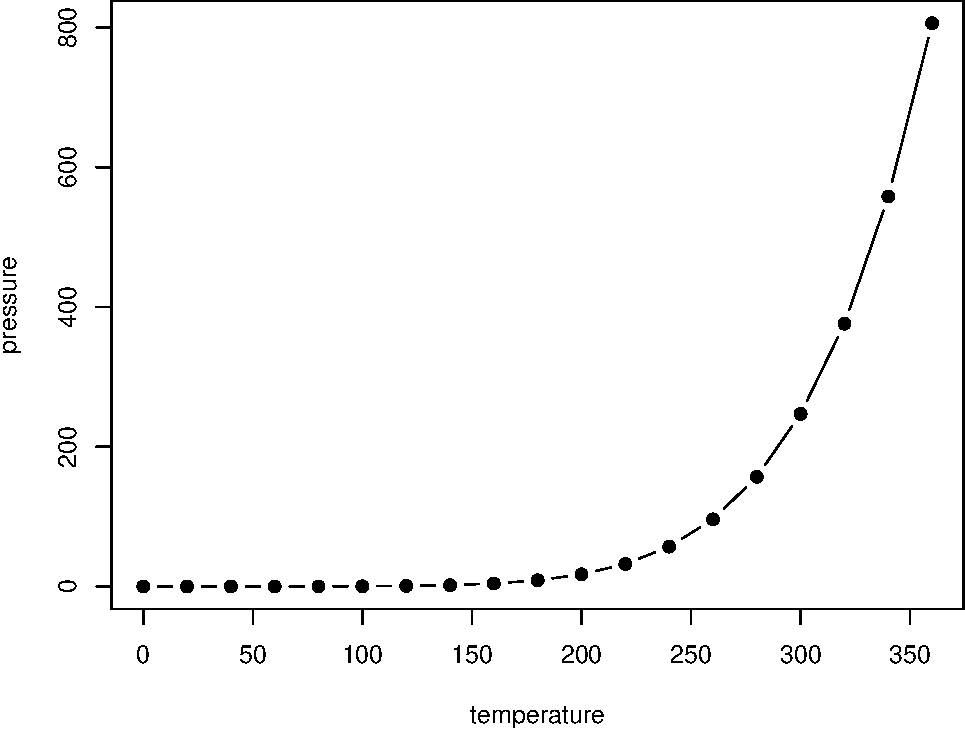
\includegraphics[width=0.8\linewidth]{BookR_files/figure-latex/nice-fig-1} 

}

\caption{Here is a nice figure!}\label{fig:nice-fig}
\end{figure}

Reference a figure by its code chunk label with the \texttt{fig:} prefix, e.g., see Figure \ref{fig:nice-fig}. Similarly, you can reference tables generated from \texttt{knitr::kable()}, e.g., see Table \ref{tab:nice-tab}.

\begin{Shaded}
\begin{Highlighting}[]
\NormalTok{knitr}\OperatorTok{::}\KeywordTok{kable}\NormalTok{(}
  \KeywordTok{head}\NormalTok{(iris, }\DecValTok{20}\NormalTok{), }\DataTypeTok{caption =} \StringTok{'Here is a nice table!'}\NormalTok{,}
  \DataTypeTok{booktabs =} \OtherTok{TRUE}
\NormalTok{)}
\end{Highlighting}
\end{Shaded}

\begin{table}

\caption{\label{tab:nice-tab}Here is a nice table!}
\centering
\begin{tabular}[t]{rrrrl}
\toprule
Sepal.Length & Sepal.Width & Petal.Length & Petal.Width & Species\\
\midrule
5.1 & 3.5 & 1.4 & 0.2 & setosa\\
4.9 & 3.0 & 1.4 & 0.2 & setosa\\
4.7 & 3.2 & 1.3 & 0.2 & setosa\\
4.6 & 3.1 & 1.5 & 0.2 & setosa\\
5.0 & 3.6 & 1.4 & 0.2 & setosa\\
\addlinespace
5.4 & 3.9 & 1.7 & 0.4 & setosa\\
4.6 & 3.4 & 1.4 & 0.3 & setosa\\
5.0 & 3.4 & 1.5 & 0.2 & setosa\\
4.4 & 2.9 & 1.4 & 0.2 & setosa\\
4.9 & 3.1 & 1.5 & 0.1 & setosa\\
\addlinespace
5.4 & 3.7 & 1.5 & 0.2 & setosa\\
4.8 & 3.4 & 1.6 & 0.2 & setosa\\
4.8 & 3.0 & 1.4 & 0.1 & setosa\\
4.3 & 3.0 & 1.1 & 0.1 & setosa\\
5.8 & 4.0 & 1.2 & 0.2 & setosa\\
\addlinespace
5.7 & 4.4 & 1.5 & 0.4 & setosa\\
5.4 & 3.9 & 1.3 & 0.4 & setosa\\
5.1 & 3.5 & 1.4 & 0.3 & setosa\\
5.7 & 3.8 & 1.7 & 0.3 & setosa\\
5.1 & 3.8 & 1.5 & 0.3 & setosa\\
\bottomrule
\end{tabular}
\end{table}

You can write citations, too. For example, we are using the \textbf{bookdown} package \citep{R-bookdown} in this sample book, which was built on top of R Markdown and \textbf{knitr} \citep{xie2015}.

\hypertarget{marcos-de-datos-y-tibbles}{%
\chapter{Marcos de datos y Tibbles}\label{marcos-de-datos-y-tibbles}}

Cree estructuras de datos tabulares con marcos de datos y vea cómo se comparan con tibbles. Extraiga vectores de columna de marcos de datos para realizar cálculos. Obtenga información de metadatos como dimensiones. Seleccione las filas superior e inferior para obtener una descripción general rápida.

\hypertarget{construye-un-marco-de-datos-a-partir-de-vectores}{%
\section{Construye un marco de datos a partir de vectores}\label{construye-un-marco-de-datos-a-partir-de-vectores}}

Los datos tabulares son el formato más común utilizado por los científicos de datos. En R, las tablas se representan mediante marcos de datos. Pueden inspeccionarse imprimiéndolos en la consola.

\begin{itemize}
\tightlist
\item
  Comprender por qué los marcos de datos son importantes
\item
  Interpretar la salida de la consola creada por un marco de datos
\item
  Cree un nuevo marco de datos usando la función \texttt{data.frame()}
\item
  Definir los vectores que se utilizarán para columnas individuales
\item
  Especificar los nombres de las columnas del marco de datos
\end{itemize}

\begin{verbatim}
data.frame(___ = ___, 
           ___ = ___, 
           ...)
\end{verbatim}

\hypertarget{introducciuxf3n-a-los-marcos-de-datos}{%
\subsection{Introducción a los marcos de datos}\label{introducciuxf3n-a-los-marcos-de-datos}}

En análisis y estadísticas, los datos tabulares son la estructura de datos más importante. Está presente en muchos formatos comunes como archivos de Excel, valores separados por comas (CSV) o bases de datos. R integra objetos de datos tabulares como ciudadanos de primera clase en el idioma a través de \emph{marcos de datos}. Los marcos de datos permiten a los usuarios leer y manipular fácilmente datos tabulares dentro del lenguaje R.

Echemos un vistazo a un objeto de marco de datos llamado \texttt{Davis}, del paquete \textbf{carData}, que incluye medidas de altura y peso para 200 hombres y mujeres:

\begin{Shaded}
\begin{Highlighting}[]
\KeywordTok{tibble}\NormalTok{ (Davis)}
\end{Highlighting}
\end{Shaded}

\begin{verbatim}
## # A tibble: 200 x 5
##    sex   weight height repwt repht
##    <fct>  <int>  <int> <int> <int>
##  1 M         77    182    77   180
##  2 F         58    161    51   159
##  3 F         53    161    54   158
##  4 M         68    177    70   175
##  5 F         59    157    59   155
##  6 M         76    170    76   165
##  7 M         76    167    77   165
##  8 M         69    186    73   180
##  9 M         71    178    71   175
## 10 M         65    171    64   170
## # ... with 190 more rows
\end{verbatim}

De la salida impresa, podemos ver que el marco de datos abarca más de 200 \textbf{filas} y 5 \textbf{columnas}. En el ejemplo anterior, cada fila contiene datos de una persona a través de \textbf{atributos}, que corresponden a las columnas \texttt{sex}, \texttt{weight}, \texttt{height}, \texttt{repwt} (peso reportado) y \texttt{repht} (altura reportado).

Por ejemplo, la primera fila de la tabla especifica un hombre que pesa \texttt{77} kg y tiene una altura de \texttt{182} cm. Los pesos reportados están muy cerca de \texttt{77} kg y \texttt{180} cm, respectivamente.

Las filas en un marco de datos se identifican además por los \emph{nombres de fila} a la izquierda, que son simplemente los números de fila por defecto. En el caso del conjunto de datos de \texttt{Davis} anterior, los nombres de las filas van de 1 a 200.

\hypertarget{crear-marcos-de-datos}{%
\subsection{Crear marcos de datos}\label{crear-marcos-de-datos}}

\begin{verbatim}
data.frame(___ = ___, 
           ___ = ___, 
           ...)
\end{verbatim}

Los marcos de datos contienen datos tabulares en varias columnas o \emph{atributos}. Cada columna está representada por un vector de diferentes \emph{tipos de datos} como números o caracteres. La función \texttt{data.frame()} admite la construcción de objetos de marco de datos combinando diferentes vectores en una tabla. Para formar una tabla, se requiere que los vectores tengan la misma longitud. Un marco de datos también puede verse como una colección de vectores conectados entre sí para formar una tabla.

Creemos nuestro primer marco de datos con cuatro personas diferentes, incluidos sus identificadores, nombres e indicadores si son mujeres o no. Cada uno de estos atributos es creado por un vector diferente de diferentes tipos de datos (numéricos, de caracteres y lógicos). Los atributos finalmente se combinan en una tabla usando la función \texttt{data.frame()}:

\begin{Shaded}
\begin{Highlighting}[]
\KeywordTok{data.frame}\NormalTok{(}
  \KeywordTok{c}\NormalTok{(}\DecValTok{1}\NormalTok{, }\DecValTok{2}\NormalTok{, }\DecValTok{3}\NormalTok{, }\DecValTok{4}\NormalTok{),}
  \KeywordTok{c}\NormalTok{(}\StringTok{"Louisa"}\NormalTok{, }\StringTok{"Jonathan"}\NormalTok{, }\StringTok{"Luigi"}\NormalTok{, }\StringTok{"Rachel"}\NormalTok{),}
  \KeywordTok{c}\NormalTok{(}\OtherTok{TRUE}\NormalTok{, }\OtherTok{FALSE}\NormalTok{, }\OtherTok{FALSE}\NormalTok{, }\OtherTok{TRUE}\NormalTok{)}
\NormalTok{)}
\end{Highlighting}
\end{Shaded}

\begin{verbatim}
##   c.1..2..3..4. c..Louisa....Jonathan....Luigi....Rachel..
## 1             1                                     Louisa
## 2             2                                   Jonathan
## 3             3                                      Luigi
## 4             4                                     Rachel
##   c.TRUE..FALSE..FALSE..TRUE.
## 1                        TRUE
## 2                       FALSE
## 3                       FALSE
## 4                        TRUE
\end{verbatim}

El marco de datos resultante almacena los valores de cada vector en una columna diferente. Tiene cuatro filas y tres columnas. Sin embargo, los nombres de las columnas impresas en la primera línea parecen incluir los valores de las columnas separados por puntos, lo cual es un esquema de nombres muy extraño.

Los nombres de columna se pueden incluir en la construcción de \texttt{data.frame()} como nombres de argumentos que preceden a los valores de los vectores de columna. Para mejorar el nombre de la columna del marco de datos anterior, podemos escribir

\begin{Shaded}
\begin{Highlighting}[]
\KeywordTok{data.frame}\NormalTok{(}
  \DataTypeTok{id =} \KeywordTok{c}\NormalTok{(}\DecValTok{1}\NormalTok{, }\DecValTok{2}\NormalTok{, }\DecValTok{3}\NormalTok{, }\DecValTok{4}\NormalTok{),}
  \DataTypeTok{name =} \KeywordTok{c}\NormalTok{(}\StringTok{"Louisa"}\NormalTok{, }\StringTok{"Jonathan"}\NormalTok{, }\StringTok{"Luigi"}\NormalTok{, }\StringTok{"Rachel"}\NormalTok{),}
  \DataTypeTok{female =} \KeywordTok{c}\NormalTok{(}\OtherTok{TRUE}\NormalTok{, }\OtherTok{FALSE}\NormalTok{, }\OtherTok{FALSE}\NormalTok{, }\OtherTok{TRUE}\NormalTok{)}
\NormalTok{)}
\end{Highlighting}
\end{Shaded}

\begin{verbatim}
##   id     name female
## 1  1   Louisa   TRUE
## 2  2 Jonathan  FALSE
## 3  3    Luigi  FALSE
## 4  4   Rachel   TRUE
\end{verbatim}

El marco de datos resultante incluye los nombres de columna necesarios para ver el significado real de las diferentes columnas.

\hypertarget{crea-y-convierte-tibbles}{%
\section{Crea y convierte tibbles}\label{crea-y-convierte-tibbles}}

Tibbles son la reimaginación moderna de marcos de datos y comparten muchos puntos en común con sus antepasados. La diferencia más visible es cómo se imprime el contenido de tibble en la consola. Tibbles son parte del tidyverse y se utilizan por su comportamiento más consistente en comparación con los marcos de datos.

\begin{itemize}
\tightlist
\item
  Conozca la diferencia entre \emph{marcos de datos} y \emph{tibbles}
\item
  Crear \emph{tibbles} a partir de vectores
\item
  Convertir \emph{marcos de datos} en tibbles
\end{itemize}

\begin{verbatim}
tibble(___ = ___, 
       ___ = ___, 
       ...)
as_tibble(___)
\end{verbatim}

\hypertarget{introducciuxf3n-a-tibbles}{%
\subsection{Introducción a Tibbles}\label{introducciuxf3n-a-tibbles}}

\begin{quote}
Una reinvención moderna del marco de datos
\url{https://tibble.tidyverse.org}
\end{quote}

Tibbles son en muchos aspectos similares a los marcos de datos. De hecho, se \emph{heredan} de los marcos de datos, lo que significa que todas las funciones y características disponibles para los marcos de datos también funcionan para tibbles. Por tanto, cuando hablamos de \emph{marcos de datos} también nos referimos a \emph{tibbles}.

Además de todo lo que ofrece un marco de datos, los tibbles tienen un comportamiento más consistente con una mejor usabilidad en muchos casos. Lo más importante es que cuando se imprime un objeto tibble en la consola, muestra automáticamente solo las primeras 10 filas y condensa columnas adicionales. Por el contrario, un marco de datos llena toda la pantalla de la consola con valores que pueden generar confusión. Echemos un vistazo al conjunto de datos \texttt{gapminder} del paquete \textbf{gapminder}:

\begin{Shaded}
\begin{Highlighting}[]
\NormalTok{gapminder}\OperatorTok{::}\NormalTok{gapminder}
\end{Highlighting}
\end{Shaded}

\begin{verbatim}
## # A tibble: 1,704 x 6
##    country     continent  year lifeExp      pop gdpPercap
##    <fct>       <fct>     <int>   <dbl>    <int>     <dbl>
##  1 Afghanistan Asia       1952    28.8  8425333      779.
##  2 Afghanistan Asia       1957    30.3  9240934      821.
##  3 Afghanistan Asia       1962    32.0 10267083      853.
##  4 Afghanistan Asia       1967    34.0 11537966      836.
##  5 Afghanistan Asia       1972    36.1 13079460      740.
##  6 Afghanistan Asia       1977    38.4 14880372      786.
##  7 Afghanistan Asia       1982    39.9 12881816      978.
##  8 Afghanistan Asia       1987    40.8 13867957      852.
##  9 Afghanistan Asia       1992    41.7 16317921      649.
## 10 Afghanistan Asia       1997    41.8 22227415      635.
## # ... with 1,694 more rows
\end{verbatim}

Inmediatamente vemos que el conjunto de datos \texttt{gapminder} es un tibble que consta de 1,704 filas y 6 columnas en la línea superior. En la segunda línea podemos ver los nombres de las columnas y sus correspondientes \emph{tipos de datos} directamente debajo.

Por ejemplo, la columna \texttt{country} tiene el tipo \texttt{\textless{}fct\textgreater{}} (que es la abreviatura de ``factor''), \texttt{year} es un número entero \texttt{\textless{}int\textgreater{}} y la esperanza de vida \texttt{lifeExp} es un \texttt{\textless{}dbl\textgreater{}}, un número decimal.

\hypertarget{creando-tibbles}{%
\subsection{Creando Tibbles}\label{creando-tibbles}}

\begin{verbatim}
tibble(___ = ___, 
       ___ = ___, 
       ...)
as_tibble(___)
\end{verbatim}

La creación de tibbles funciona exactamente igual que para los marcos de datos. Podemos usar la función \texttt{tibble()} del paquete \textbf{tibble} para crear un nuevo objeto tabular.

Por ejemplo, un tibble que contenga datos de cuatro personas diferentes y tres columnas se puede crear así:

\begin{Shaded}
\begin{Highlighting}[]
\KeywordTok{library}\NormalTok{(tibble)}
\KeywordTok{tibble}\NormalTok{(}
  \DataTypeTok{id =} \KeywordTok{c}\NormalTok{(}\DecValTok{1}\NormalTok{, }\DecValTok{2}\NormalTok{, }\DecValTok{3}\NormalTok{, }\DecValTok{4}\NormalTok{),}
  \DataTypeTok{name =} \KeywordTok{c}\NormalTok{(}\StringTok{"Louisa"}\NormalTok{, }\StringTok{"Jonathan"}\NormalTok{, }\StringTok{"Luigi"}\NormalTok{, }\StringTok{"Rachel"}\NormalTok{),}
  \DataTypeTok{female =} \KeywordTok{c}\NormalTok{(}\OtherTok{TRUE}\NormalTok{, }\OtherTok{FALSE}\NormalTok{, }\OtherTok{FALSE}\NormalTok{, }\OtherTok{TRUE}\NormalTok{)}
\NormalTok{)}
\end{Highlighting}
\end{Shaded}

\begin{verbatim}
## # A tibble: 4 x 3
##      id name     female
##   <dbl> <chr>    <lgl> 
## 1     1 Louisa   TRUE  
## 2     2 Jonathan FALSE 
## 3     3 Luigi    FALSE 
## 4     4 Rachel   TRUE
\end{verbatim}

\hypertarget{conversiuxf3n-de-marcos-de-datos-a-tibbles}{%
\subsection{Conversión de marcos de datos a Tibbles}\label{conversiuxf3n-de-marcos-de-datos-a-tibbles}}

Si prefiere tibbles a marcos de datos por sus características adicionales, también se pueden convertir a partir de marcos de datos existentes con la función \texttt{as\_tibble()}.

Por ejemplo, el marco de datos de \texttt{Davis} del paquete \textbf{carData} se puede convertir a un tibble así:

\begin{Shaded}
\begin{Highlighting}[]
\KeywordTok{as_tibble}\NormalTok{(Davis)}
\end{Highlighting}
\end{Shaded}

\begin{verbatim}
## # A tibble: 200 x 5
##    sex   weight height repwt repht
##    <fct>  <int>  <int> <int> <int>
##  1 M         77    182    77   180
##  2 F         58    161    51   159
##  3 F         53    161    54   158
##  4 M         68    177    70   175
##  5 F         59    157    59   155
##  6 M         76    170    76   165
##  7 M         76    167    77   165
##  8 M         69    186    73   180
##  9 M         71    178    71   175
## 10 M         65    171    64   170
## # ... with 190 more rows
\end{verbatim}

\hypertarget{extraiga-o-reemplace-columnas-en-un-marco-de-datos-usando}{%
\section{Extraiga o reemplace columnas en un marco de datos usando \$}\label{extraiga-o-reemplace-columnas-en-un-marco-de-datos-usando}}

Las columnas de un marco de datos se pueden extraer y manipular fácilmente con el operador \texttt{\$}. Incluso se pueden agregar nuevas columnas asignando un vector.

\begin{itemize}
\tightlist
\item
  Extraiga columnas de un marco de datos con \texttt{\$}.
\item
  Reemplazar valores de columnas existentes en un marco de datos.
\item
  Agregue nuevas columnas a un marco de datos.
\end{itemize}

\begin{verbatim}
___$___
___$___  <- ___
\end{verbatim}

\hypertarget{extraer-columnas-con}{%
\subsection{Extraer columnas con \$}\label{extraer-columnas-con}}

Los marcos de datos son tablas que resultan de la combinación de vectores de columna. Los usuarios pueden interactuar con los marcos de datos a través de numerosos operadores para extraer, agregar o recombinar valores. Para extraer columnas individuales de un marco de datos, R ofrece un operador muy específico: el dólar \texttt{\$}. Devuelve el vector de columna como lo indica su nombre basado en un marco de datos que precede a \texttt{\$}.

Para ver el operador \texttt{\$} en acción, extraigamos la población \texttt{pop} (en 1,000) de diferentes estados de los EE. UU. Según el conjunto de datos de los estados (de 1992) en el paquete \textbf{carData}:

\begin{Shaded}
\begin{Highlighting}[]
\NormalTok{carData}\OperatorTok{::}\NormalTok{States}\OperatorTok{$}\NormalTok{pop}
\end{Highlighting}
\end{Shaded}

\begin{verbatim}
##  [1]  4041   550  3665  2351 29760  3294  3287   666   607 12938  6478  1108
## [13]  1007 11431  5544  2777  2478  3685  4220  1228  4781  6016  9295  4375
## [25]  2573  5117   799  1578  1202  1109  7730  1515 17990  6629   639 10847
## [37]  3146  2842 11882  1003  3487   696  4877 16987  1723   563  6187  4867
## [49]  1793  4892   454
\end{verbatim}

El comando extrae la columna de población como vector del marco de datos. A partir de este vector podemos calcular la \texttt{sum()} de la población total como:

\begin{Shaded}
\begin{Highlighting}[]
\KeywordTok{sum}\NormalTok{(States}\OperatorTok{$}\NormalTok{pop)}
\end{Highlighting}
\end{Shaded}

\begin{verbatim}
## [1] 248709
\end{verbatim}

De manera similar, el salario promedio (en \$1,000) de los maestros se puede calcular como la \texttt{mean()} de la columna \texttt{pay}:

\begin{Shaded}
\begin{Highlighting}[]
\KeywordTok{mean}\NormalTok{(States}\OperatorTok{$}\NormalTok{pay)}
\end{Highlighting}
\end{Shaded}

\begin{verbatim}
## [1] 30.94118
\end{verbatim}

\hypertarget{determinar-el-tamauxf1o-de-un-marco-de-datos}{%
\section{Determinar el tamaño de un marco de datos}\label{determinar-el-tamauxf1o-de-un-marco-de-datos}}

El tamaño de un marco de datos, como el número de filas o columnas, a menudo es necesario y se puede determinar de varias formas.

\begin{itemize}
\tightlist
\item
  Obtener el número de filas de un marco de datos
\item
  Obtener el número de columnas de un marco de datos
\item
  Obtener dimensiones de un marco de datos
\end{itemize}

\begin{verbatim}
nrow(___)
ncol(___)
dim(___)
length(___)
\end{verbatim}

\hypertarget{dimensiones-del-marco-de-datos}{%
\subsection{Dimensiones del marco de datos}\label{dimensiones-del-marco-de-datos}}

El número de filas y columnas en un marco de datos se puede adivinar a través de la salida impresa del marco de datos. Sin embargo, es mucho más fácil obtener esta información directamente a través de funciones. Además, es posible que desee utilizar esta información en algunas partes del código.

Los marcos de datos tienen dos dimensiones. El número de filas se considera la primera dimensión. Por lo general, define el número de observaciones en un conjunto de datos. Para obtener el número de filas del marco de datos de \texttt{Davis} en el conjunto de datos \textbf{carData}, use la función \texttt{nrow()}:

\begin{Shaded}
\begin{Highlighting}[]
\KeywordTok{nrow}\NormalTok{(Davis)}
\end{Highlighting}
\end{Shaded}

\begin{verbatim}
## [1] 200
\end{verbatim}

De manera similar, el número de columnas o \emph{atributos} del marco de datos se puede recuperar con \texttt{ncol()}:

\begin{Shaded}
\begin{Highlighting}[]
\KeywordTok{ncol}\NormalTok{(Davis)}
\end{Highlighting}
\end{Shaded}

\begin{verbatim}
## [1] 5
\end{verbatim}

\hypertarget{recuperar-las-dimensiones-del-marco-de-datos}{%
\subsection{Recuperar las dimensiones del marco de datos}\label{recuperar-las-dimensiones-del-marco-de-datos}}

Para recuperar el tamaño de todas las dimensiones de un marco de datos a la vez, puede usar la función \texttt{dim()}. \texttt{dim()} devuelve un vector con dos elementos, el primer elemento es el número de filas y el segundo elemento el número de columnas.

Por ejemplo, las dimensiones del conjunto de datos de \texttt{Davis} se pueden recuperar como:

\begin{Shaded}
\begin{Highlighting}[]
\KeywordTok{dim}\NormalTok{(Davis)}
\end{Highlighting}
\end{Shaded}

\begin{verbatim}
## [1] 200   5
\end{verbatim}

Además de los marcos de datos, \texttt{dim()} también se puede utilizar para otros objetos R multidimensionales, como matrices. Sin embargo, cuando se usa con vectores \texttt{dim} solo devuelve \texttt{NULL}:

\begin{Shaded}
\begin{Highlighting}[]
\KeywordTok{dim}\NormalTok{(}\KeywordTok{c}\NormalTok{(}\DecValTok{1}\NormalTok{, }\DecValTok{3}\NormalTok{, }\DecValTok{5}\NormalTok{, }\DecValTok{7}\NormalTok{))}
\end{Highlighting}
\end{Shaded}

\begin{verbatim}
## NULL
\end{verbatim}

En cambio, la longitud de un vector se determina mediante \texttt{length()}:

\begin{Shaded}
\begin{Highlighting}[]
\KeywordTok{length}\NormalTok{(}\KeywordTok{c}\NormalTok{(}\DecValTok{1}\NormalTok{, }\DecValTok{3}\NormalTok{, }\DecValTok{5}\NormalTok{, }\DecValTok{7}\NormalTok{))}
\end{Highlighting}
\end{Shaded}

\begin{verbatim}
## [1] 4
\end{verbatim}

En el caso de un marco de datos, \texttt{length()} devuelve su número de columnas:

\begin{Shaded}
\begin{Highlighting}[]
\KeywordTok{length}\NormalTok{(Davis)}
\end{Highlighting}
\end{Shaded}

\begin{verbatim}
## [1] 5
\end{verbatim}

\hypertarget{seleccionar-la-primera-o-la-uxfaltima-fila-de-un-marco-de-datos}{%
\section{Seleccionar la primera o la última fila de un marco de datos}\label{seleccionar-la-primera-o-la-uxfaltima-fila-de-un-marco-de-datos}}

A menudo no necesitamos mirar todo el contenido de un marco de datos en la consola. En cambio, solo algunas partes son suficientes, como la parte superior o inferior recuperada a través de las funciones \texttt{head()} y \texttt{tail()}.

\begin{itemize}
\tightlist
\item
  Seleccionar la parte superior de un marco de datos
\item
  Seleccione la parte inferior de un marco de datos
\item
  Especifique el número de líneas a seleccionar mediante el parámetro n
\end{itemize}

\begin{verbatim}
head(___, n = ___)
tail(___, n = ___)
\end{verbatim}

\hypertarget{seleccionar-la-parte-superior-de-un-marco-de-datos}{%
\subsection{Seleccionar la parte superior de un marco de datos}\label{seleccionar-la-parte-superior-de-un-marco-de-datos}}

Los marcos de datos pueden abarcar una gran cantidad de filas y columnas. Según la salida impresa en la consola, puede ser difícil obtener una impresión inicial de los datos dentro del marco de datos. Este problema no es tanto un problema para tibbles que tienen una mejor salida de consola. Además, puede ser útil recuperar fácilmente las primeras filas en un comando sin indexación ni paquetes adicionales.

El conjunto de datos \texttt{TitanicSurvival} contiene datos de 1309 pasajeros representados como filas. Una simple impresión del conjunto de datos imprimiría a todos los pasajeros, llenando toda la consola. En cambio, la función \texttt{head()} muestra solo las primeras 10 filas de un marco de datos, incluidos los nombres de sus columnas:

\begin{Shaded}
\begin{Highlighting}[]
\KeywordTok{head}\NormalTok{(TitanicSurvival)}
\end{Highlighting}
\end{Shaded}

\begin{verbatim}
##                                 survived    sex     age passengerClass
## Allen, Miss. Elisabeth Walton        yes female 29.0000            1st
## Allison, Master. Hudson Trevor       yes   male  0.9167            1st
## Allison, Miss. Helen Loraine          no female  2.0000            1st
## Allison, Mr. Hudson Joshua Crei       no   male 30.0000            1st
## Allison, Mrs. Hudson J C (Bessi       no female 25.0000            1st
## Anderson, Mr. Harry                  yes   male 48.0000            1st
\end{verbatim}

El número de columnas se puede ajustar mediante el parámetro \texttt{n}. Para extraer solo las primeras tres filas del conjunto de datos, puede escribir:

\begin{Shaded}
\begin{Highlighting}[]
\KeywordTok{head}\NormalTok{(TitanicSurvival, }\DataTypeTok{n =} \DecValTok{3}\NormalTok{)}
\end{Highlighting}
\end{Shaded}

\begin{verbatim}
##                                survived    sex     age passengerClass
## Allen, Miss. Elisabeth Walton       yes female 29.0000            1st
## Allison, Master. Hudson Trevor      yes   male  0.9167            1st
## Allison, Miss. Helen Loraine         no female  2.0000            1st
\end{verbatim}

\hypertarget{seleccionar-la-parte-inferior-de-un-marco-de-datos}{%
\subsection{Seleccionar la parte inferior de un marco de datos}\label{seleccionar-la-parte-inferior-de-un-marco-de-datos}}

La función \texttt{tail()} se puede utilizar para seleccionar las filas inferiores de un marco de datos. Similar a la función \texttt{head()}, también acepta un parámetro \texttt{n} para especificar el número de filas que se devolverán.

Por ejemplo, para seleccionar las últimas cinco filas del conjunto de datos \texttt{TitanicSurvival}, puede escribir:

\begin{Shaded}
\begin{Highlighting}[]
\KeywordTok{tail}\NormalTok{(TitanicSurvival, }\DataTypeTok{n =} \DecValTok{5}\NormalTok{)}
\end{Highlighting}
\end{Shaded}

\begin{verbatim}
##                           survived    sex  age passengerClass
## Zabour, Miss. Hileni            no female 14.5            3rd
## Zabour, Miss. Thamine           no female   NA            3rd
## Zakarian, Mr. Mapriededer       no   male 26.5            3rd
## Zakarian, Mr. Ortin             no   male 27.0            3rd
## Zimmerman, Mr. Leo              no   male 29.0            3rd
\end{verbatim}

Las funciones de cabeza y cola también se pueden combinar para seleccionar un fragmento del conjunto de datos del medio. Para seleccionar las primeras cinco filas de las 500 filas inferiores, puede escribir:

\begin{Shaded}
\begin{Highlighting}[]
\KeywordTok{head}\NormalTok{(}\KeywordTok{tail}\NormalTok{(TitanicSurvival, }\DataTypeTok{n =} \DecValTok{500}\NormalTok{), }\DataTypeTok{n =} \DecValTok{5}\NormalTok{)}
\end{Highlighting}
\end{Shaded}

\begin{verbatim}
##                                 survived    sex age passengerClass
## Ford, Mr. Edward Watson               no   male  18            3rd
## Ford, Mr. William Neal                no   male  16            3rd
## Ford, Mrs. Edward (Margaret Ann       no female  48            3rd
## Fox, Mr. Patrick                      no   male  NA            3rd
## Franklin, Mr. Charles (Charles        no   male  NA            3rd
\end{verbatim}

\hypertarget{methods}{%
\chapter{Methods}\label{methods}}

We describe our methods in this chapter.

\hypertarget{introducciuxf3n-a-machine-learning}{%
\chapter{Introducción a Machine Learning}\label{introducciuxf3n-a-machine-learning}}

Aprenda los fundamentos del aprendizaje automático, incluidos casos de uso y diferentes técnicas de aprendizaje. Diferenciar entre regresión y clasificación.

¿Qué es Machine Learning?

En los últimos años, términos como inteligencia artificial, aprendizaje automático y aprendizaje profundo se han utilizado mucho. Tan misteriosas como suenan estas palabras, ¿cuál es su diferencia y de qué son capaces?

\begin{itemize}
\tightlist
\item
  Diferenciar entre inteligencia artificial, aprendizaje automático y aprendizaje profundo
\item
  Identificar casos de uso de Machine Learning
\end{itemize}

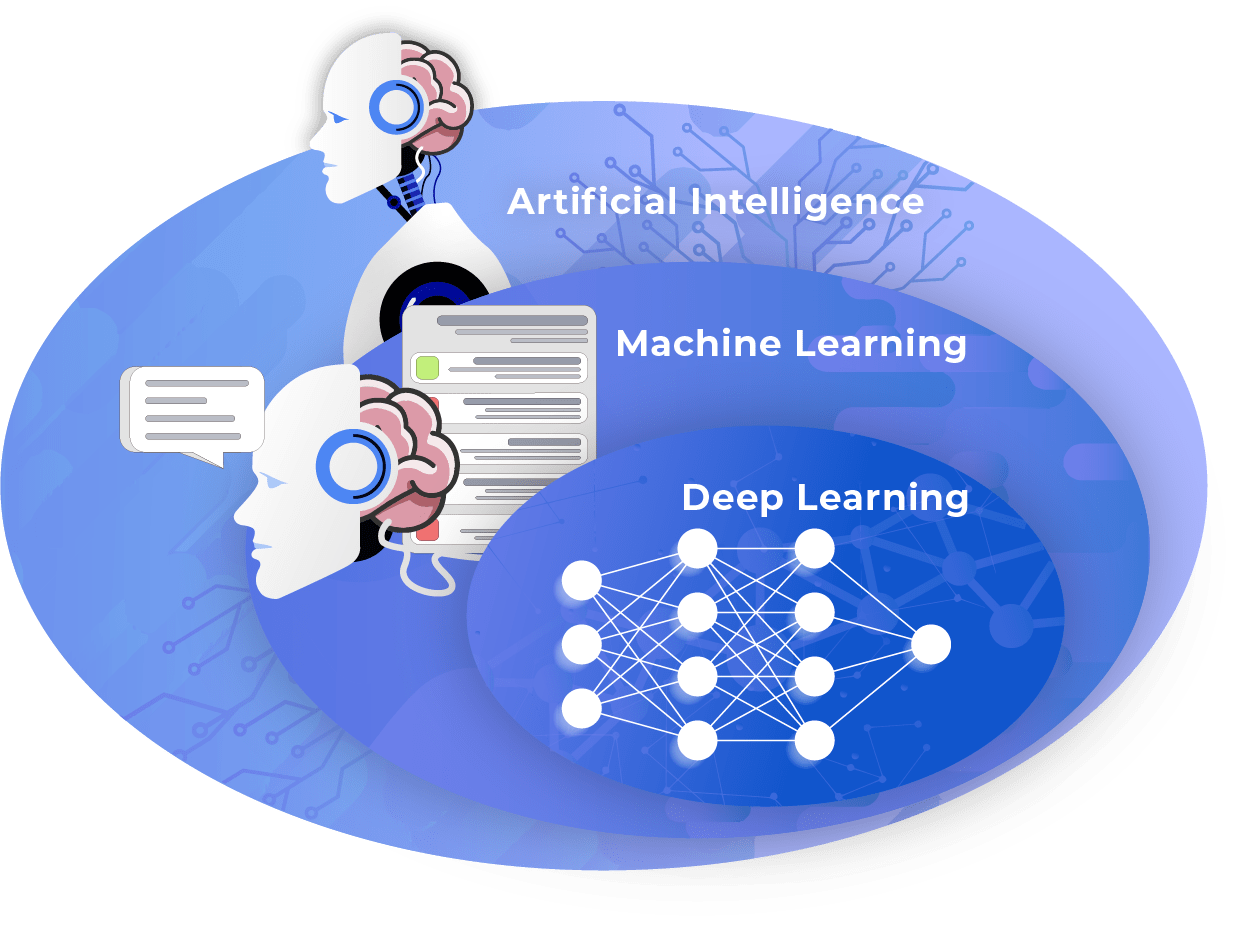
\includegraphics{img/int.png}

\hypertarget{inteligencia-artificial}{%
\section{Inteligencia artificial}\label{inteligencia-artificial}}

La \textbf{inteligencia artificial (IA)} es la inteligencia demostrada por las máquinas, en contraste con la inteligencia natural asociada con los humanos. Por inteligencia, generalmente nos referimos a la resolución de problemas y tareas complejos, que aparentemente requieren algún tipo de habilidades cognitivas. La inteligencia artificial comenzó como una disciplina académica en la década de 1950 con el supuesto de que las computadoras pueden imitar el complejo razonamiento dentro del cerebro humano. Este campo también se conoce como \emph{inteligencia artificial general (AGI)} y el objetivo de alcanzar una inteligencia similar a la humana, incluso hoy, parece estar fuera de alcance.

Sin embargo, surgió un subcampo llamado aprendizaje automático \emph{machine learning (ML)} que se centra en problemas más específicos, como el reconocimiento de imágenes o la comprensión del lenguaje. Gracias a las aplicaciones de la industria, el aprendizaje automático se ha vuelto cada vez más popular y atrae a investigadores e inversores a nivel mundial.

\hypertarget{machine-learning-aprendizaje-automuxe1tico}{%
\section{Machine Learning (Aprendizaje automático)}\label{machine-learning-aprendizaje-automuxe1tico}}

El \textbf{machine learning (ML)} es un subcampo de la inteligencia artificial. Su objetivo es construir y aplicar modelos sofisticados sin la necesidad de reglas e instrucciones codificadas. En cambio, los modelos pueden extraer reglas y patrones de los datos y aplicarlos para nuevos problemas.

La recopilación de datos, la anotación y el procesamiento previo son requisitos previos esenciales para crear modelos de aprendizaje automático. Como regla general, cuanto mayor es la complejidad de un modelo, normalmente se necesitan más datos para el entrenamiento y la validación.

Por ejemplo, podría pensar en asistentes virtuales avanzados, como \href{https://developer.amazon.com/alexa}{Alexa} (Amazon) o \href{https://www.apple.com/siri}{Siri} (Apple), que aplican el aprendizaje automático para interpretar el lenguaje natural y predecir la mejor respuesta o reacción.

\hypertarget{aprendizaje-profundo-deep-learning}{%
\section{Aprendizaje profundo (Deep Learning)}\label{aprendizaje-profundo-deep-learning}}

El \textbf{aprendizaje profundo} es un área del aprendizaje automático, que cubre únicamente las redes neuronales. El nombre de red neuronal se inspiró en el hecho de que la arquitectura modela libremente el cerebro humano. Esta técnica demostró ser especialmente adecuada para ciertas tareas como el reconocimiento de imágenes, que es la piedra angular de aplicaciones como los vehículos autónomos.

Las redes neuronales profundas son actualmente el área de investigación más candente en toda la comunidad de IA. Su popularidad se basa en muchos avances en los últimos años, incluida la competencia ImageNet que clasifica imágenes en color de alta resolución en 1000 categorías diferentes y 1,2 (1,4) millones de muestras de entrenamiento. Las redes neuronales profundas también llevaron a avances en otras áreas en las que se desempeñaron comparables o incluso mejores que sus contrapartes humanas, incluido el reconocimiento de voz, la transcripción de escritura a mano (OCR), la traducción automática, la conducción autónoma, Go playing y muchos más.

\hypertarget{casos-de-uso-populares}{%
\section{Casos de uso populares}\label{casos-de-uso-populares}}

A medida que avanzaba el campo del aprendizaje automático y las computadoras se volvían cada vez más poderosas, se habilitaron nuevas soluciones que afectaron a casi todos los campos (científicos). Hoy en día, el aprendizaje automático ayuda a los científicos a realizar diagnósticos médicos, descubrir nuevos medicamentos, monitorear la superficie de la tierra y detectar incendios forestales, automatizar y optimizar procesos en la industria financiera, etc.

Aparte de estas aplicaciones de vanguardia, a menudo tendemos a pasar por alto que el aprendizaje automático también forma parte de nuestra vida diaria. En las siguientes secciones abordaremos estas aplicaciones de aprendizaje automático y nos centraremos en sistemas como:

\begin{itemize}
\tightlist
\item
  Sistemas de recomendación
\item
  Los motores de búsqueda
\item
  Máquina traductora
\item
  Identificación de música
\item
  Autos autónomos
\end{itemize}

\hypertarget{caso-de-uso-motores-de-buxfasqueda-y-sistemas-de-recomendaciuxf3n}{%
\subsection{Caso de uso: motores de búsqueda y sistemas de recomendación}\label{caso-de-uso-motores-de-buxfasqueda-y-sistemas-de-recomendaciuxf3n}}

Los \textbf{motores de búsqueda}, como Google, aplican el aprendizaje automático de muchas formas para brindar mejores servicios. Al escribir una consulta, por ejemplo, el aprendizaje automático proporciona sugerencias de autocompletado. Estas sugerencias se personalizan en función de los temas de tendencia actual, pero también de nuestra ubicación y búsquedas anteriores. Posteriormente, las consultas se evalúan en muchos niveles para determinar nuestras intenciones exactas y clasificar los resultados en consecuencia.

De manera similar, el aprendizaje automático determina lo que se nos recomienda en YouTube, Netflix, Amazon, etc. (un campo del aprendizaje automático, a menudo denominado \textbf{sistemas de recomendación}). Estas aplicaciones predicen nuestros intereses al analizar nuestras actividades en línea. Los artículos que hemos buscado, las películas que hemos visto, los productos que hemos comprado son todos predictores sobre nuestro comportamiento e intereses futuros.

\hypertarget{caso-de-uso-traducciuxf3n-automuxe1tica}{%
\subsection{Caso de uso: traducción automática}\label{caso-de-uso-traducciuxf3n-automuxe1tica}}

Los servicios de \textbf{traducción} como \href{https://www.deepl.com/en/translator}{DeepL} también aplican cada vez más el aprendizaje automático. La idea principal detrás de estos servicios es pasar de diccionarios simples a traductores complejos que se enfocan en el contexto e interpretan el texto como un todo. El aprendizaje automático en esta configuración se puede utilizar para crear modelos que describan cómo se expresan ciertas ideas en otros lenguajes. Esto permite una comprensión más matizada del texto escrito y proporciona traducciones más naturales. Un aspecto importante de estas soluciones es que se pueden mejorar constantemente proporcionándoles nuevos ejemplos y comentarios de los que aprender.

\hypertarget{caso-de-uso-identificaciuxf3n-de-muxfasica-y-reconocimiento-de-voz}{%
\subsection{Caso de uso: identificación de música y reconocimiento de voz}\label{caso-de-uso-identificaciuxf3n-de-muxfasica-y-reconocimiento-de-voz}}

El análisis de audio es un campo propio en el aprendizaje automático. Una herramienta común en este campo es transformar señales de audio en componentes de frecuencia. En el caso de los discos de música, la composición de estos componentes de frecuencia es tan única, que podemos definir las llamadas \emph{huellas digitales} para cada canción. Esto habilita aplicaciones de \textbf{identificación de música} como Shazam, que pueden identificar y unir canciones con precisión basándose en una muestra de solo unos segundos de duración. Del mismo modo, las aplicaciones de \textbf{reconocimiento de voz} pueden identificar fácilmente las palabras habladas y convertirlas en lenguaje escrito.

\hypertarget{caso-de-uso-coches-autuxf3nomos}{%
\subsection{Caso de uso: coches autónomos}\label{caso-de-uso-coches-autuxf3nomos}}

Los \textbf{coches autónomos} como Google Waymo y Tesla dependen en gran medida del aprendizaje automático. Al analizar los datos provenientes de varios sensores, el aprendizaje automático controla la aceleración, frenado y dirección del automóvil. Estas instrucciones se basan no solo en las normas de tráfico y las señales de tráfico, sino que incluyen un modelo predictivo continuo para evitar posibles accidentes. Aunque los modelos finales de aprendizaje automático son capaces de evaluar los datos de entrada y tomar decisiones en fracciones de segundo, el entrenamiento de los modelos requiere inmensas cantidades de datos, poder computacional y tiempo.

\hypertarget{tuxe9cnicas-de-machine-learning}{%
\section{Técnicas de Machine Learning}\label{tuxe9cnicas-de-machine-learning}}

En este capítulo

\begin{itemize}
\tightlist
\item
  Familiarízate con diferentes enfoques de machine learning
\item
  Diferenciar entre técnicas de aprendizaje supervisado, no supervisado y por refuerzo.
\item
  Vea cómo se pueden aplicar las técnicas de aprendizaje para diferentes casos de uso
\end{itemize}

La idea básica del aprendizaje automático es crear modelos que se puedan utilizar para hacer predicciones y tomar decisiones. Diferenciamos entre 3 tipos de aprendizaje automático, cada uno de ellos tiene como objetivo resolver diferentes tipos de tareas: \textbf{supervisado}, \textbf{no supervisado} y \textbf{aprendizaje reforzado}.

El \textbf{aprendizaje supervisado} tiene como objetivo aprender de un conjunto de datos de ejemplo. Nuestra suposición inicial es que el valor de un resultado conocido (por ejemplo, el cliente compra un producto) está influenciado por un conjunto de entradas medibles (edad, intereses, últimos clics). Utilizando algoritmos de aprendizaje automático, intentamos detectar y modelar estas relaciones.

El \textbf{aprendizaje no supervisado} también requiere datos de entrada, pero no existe una variable de resultado predefinida. En su lugar, tratamos de detectar patrones y establecer relaciones dentro de los datos (por ejemplo, a través de agrupaciones) o reducir dimensiones (por ejemplo, con análisis de componentes principales).

El \textbf{aprendizaje reforzado} no requiere observaciones de entrada, sino un objetivo y un entorno en el que operar. Al integrar la retroalimentación continua del entorno, esperamos que el sistema cree sus propias tácticas para lograr el objetivo.

\hypertarget{aprendizaje-supervisado}{%
\subsection{Aprendizaje supervisado}\label{aprendizaje-supervisado}}

En el \emph{aprendizaje supervisado}, la variable de resultado debe conocerse para el entrenamiento de modelos. Como ejemplo, podría pensar en un modelo para la predicción de precios de apartamentos. Este modelo podría ayudar a los agentes inmobiliarios a fijar el precio de los nuevos apartamentos que ingresan al mercado. Además, los valores previstos se pueden comparar con los precios del mercado para determinar las oportunidades de compra de los apartamentos más infravalorados. Las variables de entrada requeridas para este problema probablemente incluirían aspectos como:

\begin{itemize}
\tightlist
\item
  \textbf{Ciudad}: Ubicación del apartamento por ciudad.
\item
  \textbf{Habitaciones}: Número de habitaciones del apartamento.
\item
  \textbf{Tamaño}: Tamaño del apartamento por metros cuadrados.
\end{itemize}

Como punto de partida, necesitamos un conjunto de datos con varios ejemplos que contengan esta información:

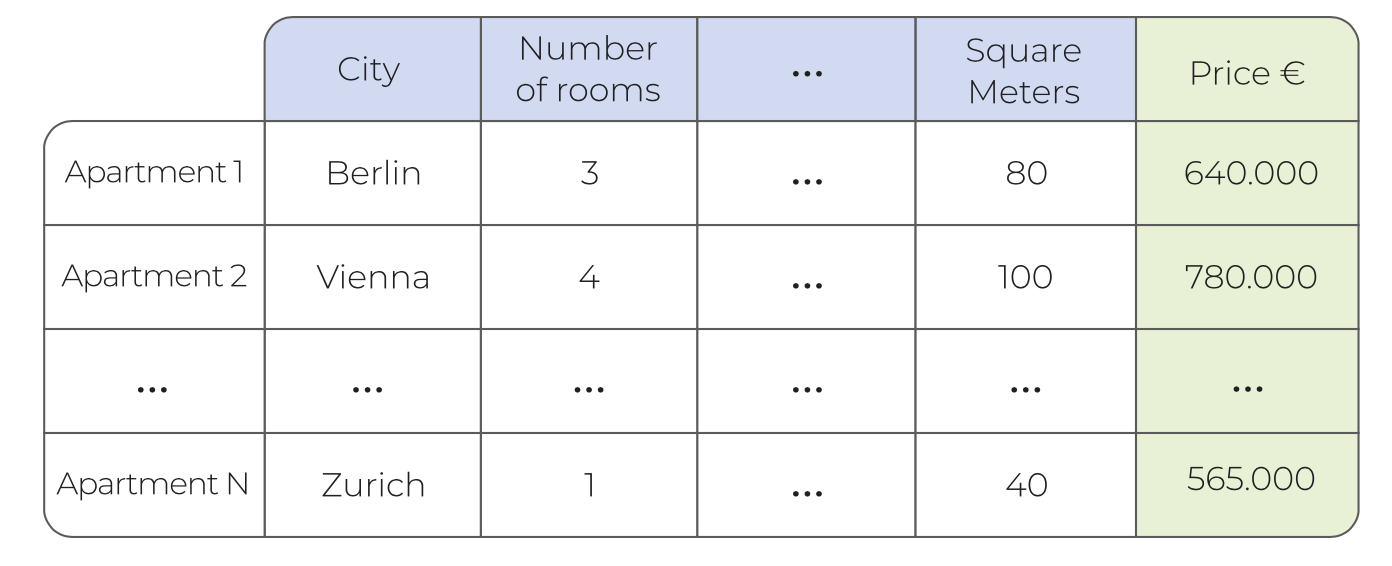
\includegraphics{img/tab1.png}

\hypertarget{aprendizaje-supervisado-objetivo}{%
\subsection{Aprendizaje supervisado: objetivo}\label{aprendizaje-supervisado-objetivo}}

El objetivo del aprendizaje automático supervisado es tomar un conjunto de ejemplos y entrenar un modelo utilizando métodos estadísticos. Este modelo debe explicar la relación entre las variables de entrada (por ejemplo, ciudad, habitaciones, tamaño) y la variable de salida (por ejemplo, precio) con la mayor precisión posible. Una vez que se ha entrenado el modelo, se puede utilizar para predecir el resultado de nuevas combinaciones de valores de entrada invisibles.

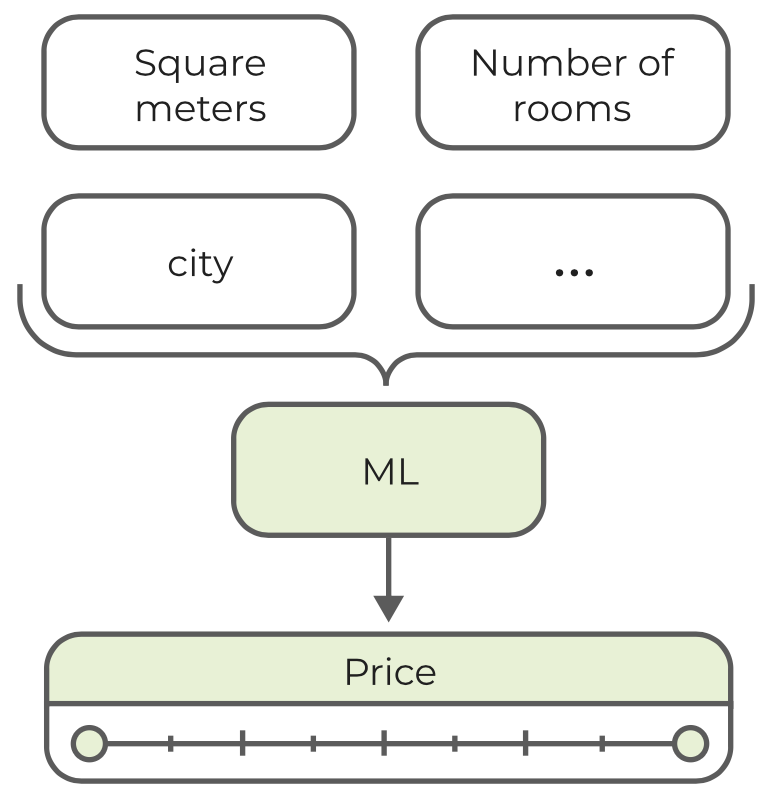
\includegraphics{img/sup.png}

\hypertarget{aprendizaje-no-supervisado}{%
\subsection{Aprendizaje no supervisado}\label{aprendizaje-no-supervisado}}

Las técnicas de aprendizaje no supervisadas extraen estructuras y patrones estadísticos de conjuntos de datos. A diferencia del aprendizaje supervisado, estas técnicas no requieren una variable de resultado predefinida en la que recibir entrenamiento.

El método de aprendizaje no supervisado más importante es la \textbf{agrupación} o cluster. La agrupación intenta agrupar las observaciones en función de su similitud. Primero, la similitud entre las observaciones se calcula como una distancia entre sí. Basándonos en estos valores, podemos determinar conglomerados (grupos) en los que las observaciones están más próximas entre sí.

\hypertarget{aprendizaje-no-supervisado-ejemplo}{%
\subsubsection{Aprendizaje no supervisado: ejemplo}\label{aprendizaje-no-supervisado-ejemplo}}

Los métodos de agrupación en clústeres se aplican a menudo como un intento de definir grupos de clientes que son similares. La similitud puede significar intereses coincidentes, datos demográficos, ubicación geográfica, etc. Esta aplicación se denomina segmentación de mercado. El objetivo de este caso de uso es comprender mejor la base de clientes y sus necesidades. Los clústeres se pueden utilizar para proporcionar anuncios y ofertas dirigidos a los clientes de acuerdo con sus propiedades. Como ejemplo, echemos un vistazo al siguiente gráfico:

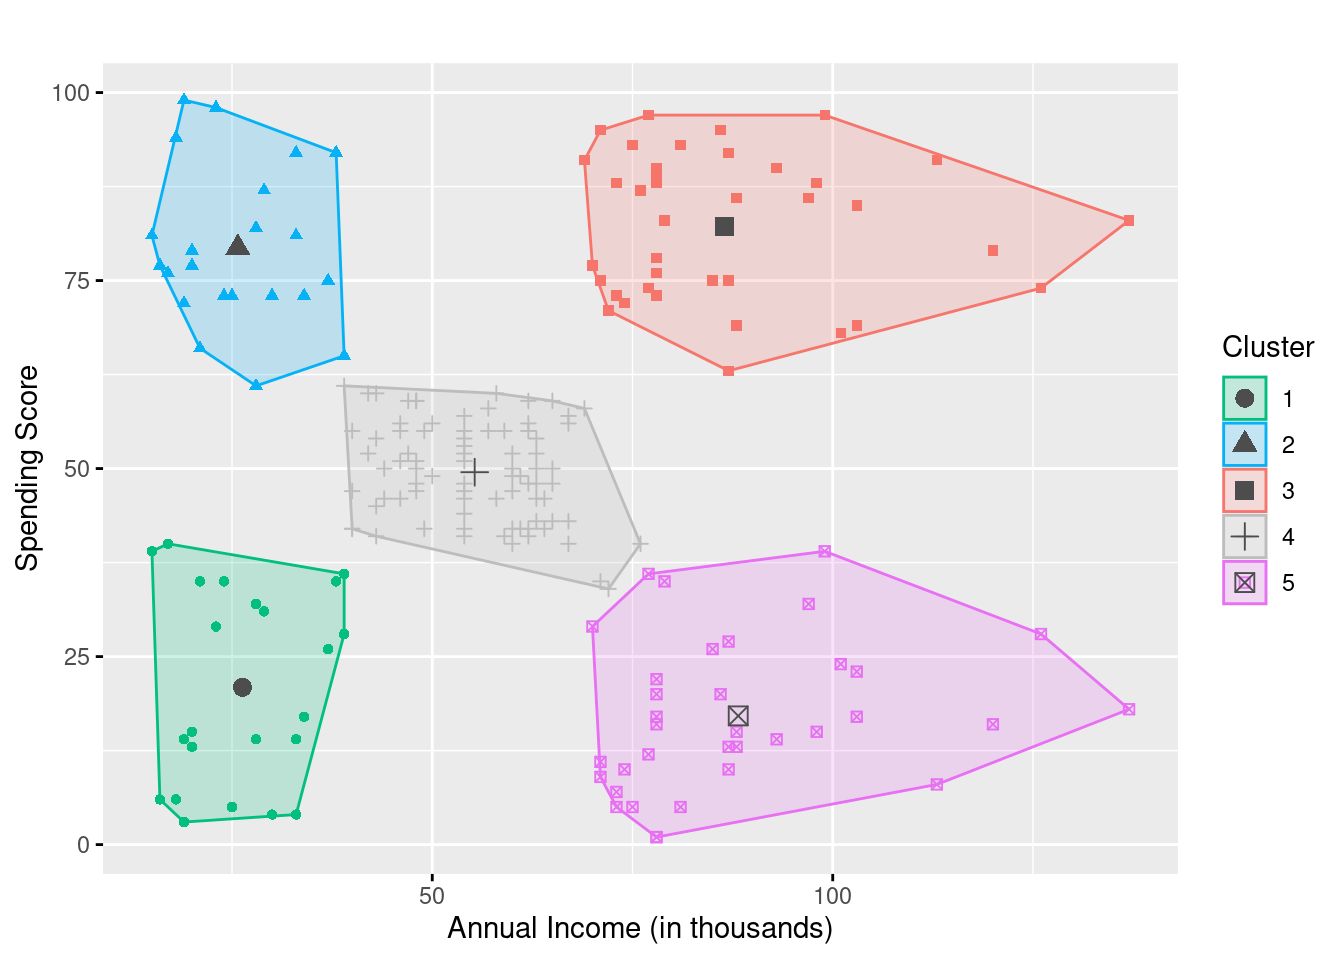
\includegraphics{img/cluster.png}
Esta gráfica compara el \texttt{Annual\ Income} y \texttt{Spending\ Score} de algunos clientes de centros comerciales. Al aplicar un algoritmo de agrupación en clústeres y definir cinco grupos, podemos separar muy bien 5 tipos diferentes de clientes. Los grupos clave en este ejemplo serían el grupo azul y rojo, que generan la mayor cantidad de ingresos. Éstos definen dos tipos de clientes. Mientras que el grupo azul contiene clientes con ingresos más bajos, el grupo rojo contiene clientes con ingresos relativamente altos. Con base en esta información, se podría adaptar la estrategia de marketing:

\begin{itemize}
\tightlist
\item
  Los clientes del clúster azul podrían ser un grupo objetivo óptimo para opciones atractivas de financiamiento y crédito.
\item
  Los clientes del grupo rojo deben mantenerse como clientes el mayor tiempo posible. En particular, debe evitarse que cambien a competidores. Por lo tanto, podrían ser un grupo objetivo óptimo para recompensas y ofertas basadas en la lealtad.
\end{itemize}

\hypertarget{aprendizaje-reforzado}{%
\subsection{Aprendizaje reforzado}\label{aprendizaje-reforzado}}

En lugar de aprender de un conjunto de ejemplos, el aprendizaje por refuerzo se basa en las recompensas acumulativas que recibe una entidad virtual (a menudo denominada \textbf{agente}) al actuar en un entorno específico. El agente intenta maximizar las recompensas acumulativas tomando decisiones. Estas decisiones se basan inicialmente en prueba y error, sin embargo, el agente se ve recompensado al tomar buenas decisiones y aprende de ellas. Del mismo modo, también existen algunos costos asociados con las malas decisiones. Por lo tanto, al crear el entorno de aprendizaje, definimos las reglas y las recompensas (y los costos), pero dejamos que el agente descubra los mejores pasos y tácticas.

\hypertarget{aprendizaje-por-refuerzo-ejemplo}{%
\subsubsection{Aprendizaje por refuerzo: ejemplo}\label{aprendizaje-por-refuerzo-ejemplo}}

Un ejemplo común es un mundo de cuadrícula, en el que el agente puede moverse de un campo a otro, excepto por posibles obstáculos o paredes, y es recompensado por encontrar la meta. Inicialmente, cada paso se daría al azar, pero después de suficientes intentos, el agente siempre iría en la dirección que maximiza sus posibilidades de obtener una recompensa. Cada paso también está asociado con un costo que reduce la recompensa acumulada. Esto significa que, desde cualquier punto de partida o posición, el agente aprendería el camino más corto hacia la recompensa después de un tiempo.

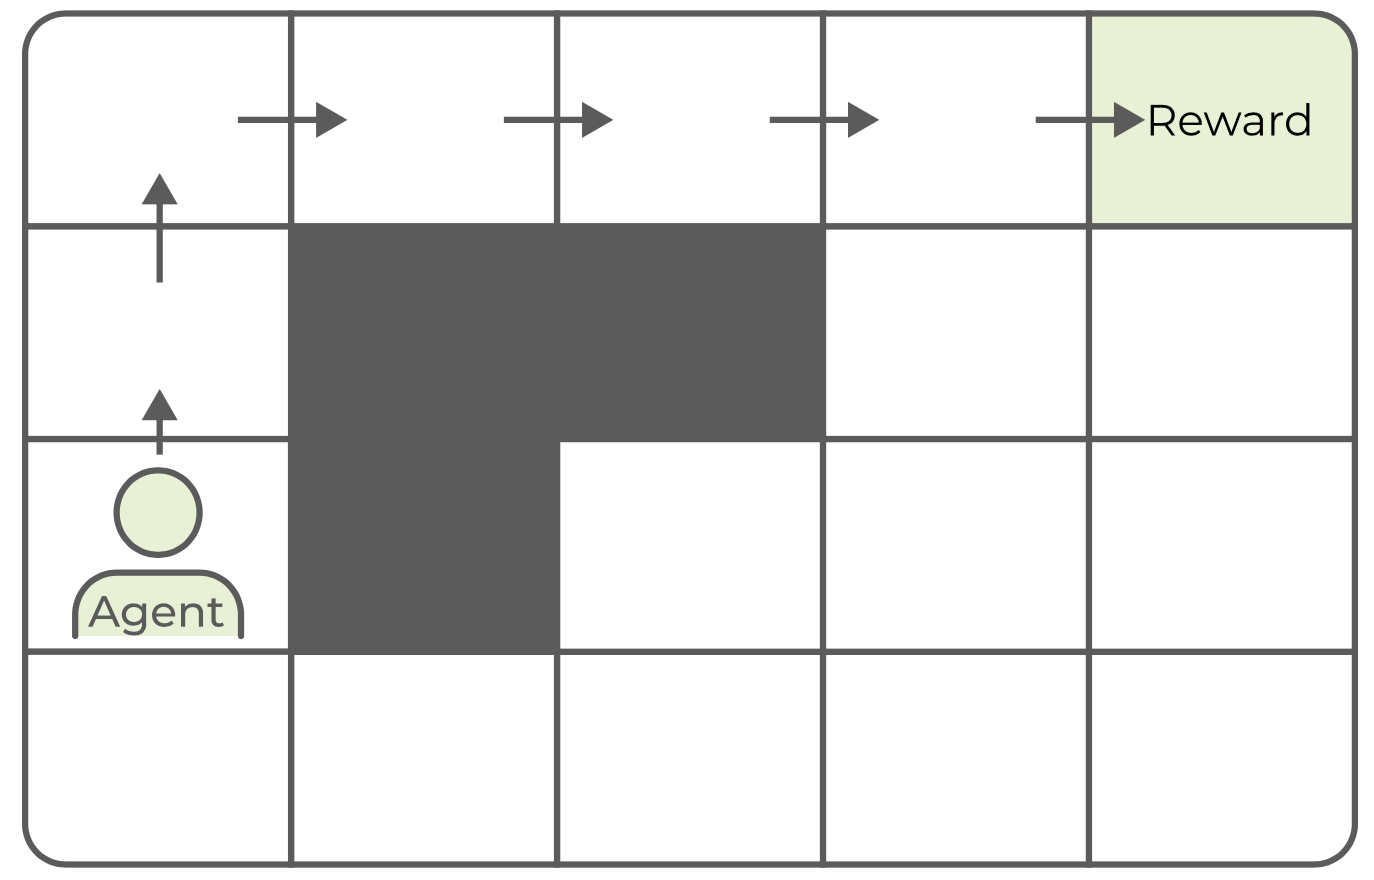
\includegraphics{img/fs.png}

\hypertarget{aprendizaje-supervisado-con-regresiuxf3n-y-clasificaciuxf3n}{%
\section{Aprendizaje supervisado con regresión y clasificación}\label{aprendizaje-supervisado-con-regresiuxf3n-y-clasificaciuxf3n}}

En el aprendizaje automático supervisado, tomamos un conjunto de observaciones con una variable de resultado conocida y entrenamos un modelo que describe con precisión la relación entre las variables de entrada y el resultado.

\begin{itemize}
\tightlist
\item
  Saber qué predictores y variables de resultado son
\item
  Diferenciar entre regresión y clasificación
\end{itemize}

\hypertarget{aprendizaje-supervisado-datos-de-entrada}{%
\subsection{Aprendizaje supervisado: datos de entrada}\label{aprendizaje-supervisado-datos-de-entrada}}

En el aprendizaje supervisado, entrenamos modelos en un conjunto de datos para describir la relación entre un valor de interés (resultado) utilizando un conjunto de valores de entrada conocidos. Por lo tanto, nuestros datos de entrenamiento para construir el modelo deben incluir todas las entradas requeridas, así como el resultado previsto en forma tabular. La tabla consta de dos partes:

\begin{enumerate}
\def\labelenumi{\arabic{enumi}.}
\tightlist
\item
  Los \textbf{predictores} o variables de entrada, que se utilizan para calcular la predicción (también conocida como matriz de modelo).
\item
  La variable de \textbf{resultado}.
\end{enumerate}

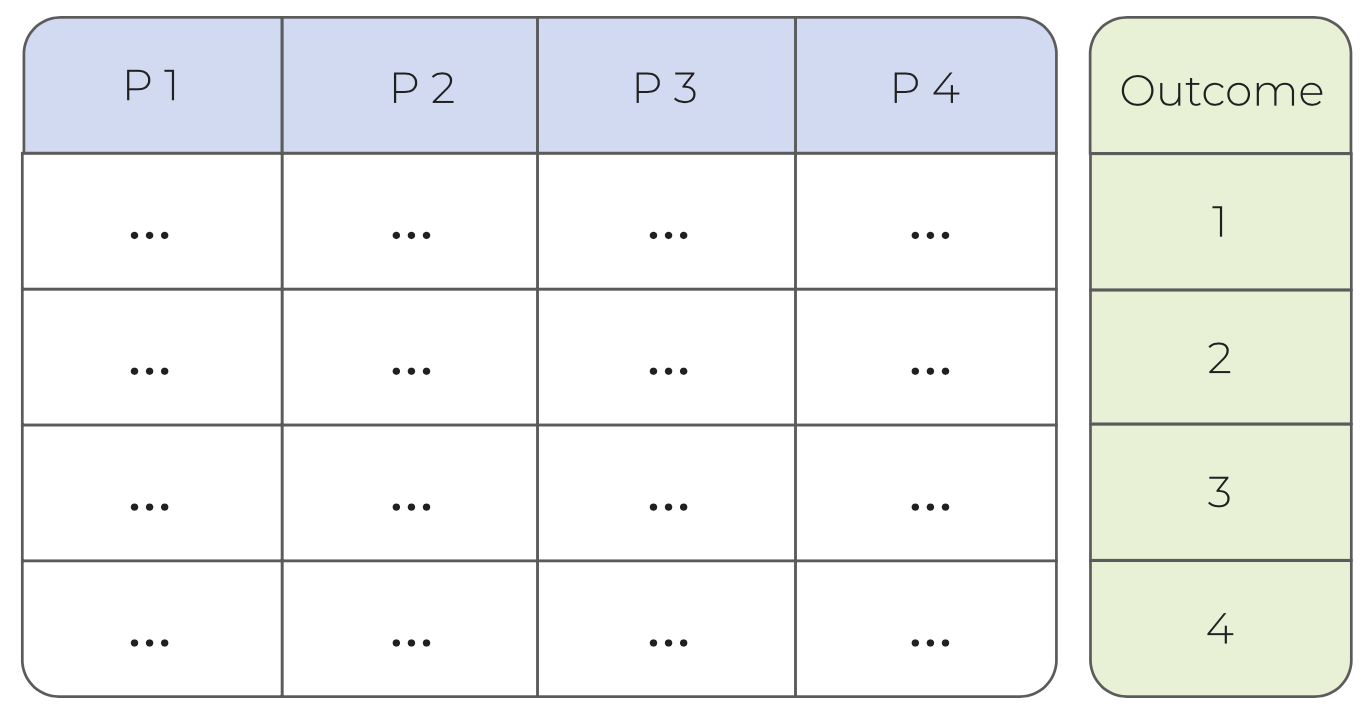
\includegraphics{img/tab.png}

\hypertarget{predictores}{%
\subsection{Predictores}\label{predictores}}

Los \textbf{predictores} son un conjunto de variables de entrada (columnas) que se utilizan para explicar y predecir el resultado. A menudo se les llama variables de \emph{entrada}, \emph{independientes}, \emph{explicativas} o simplemente \emph{características}. En el caso de los precios de los apartamentos, podría pensar en la cantidad de habitaciones, metros cuadrados o el nombre de la ciudad.

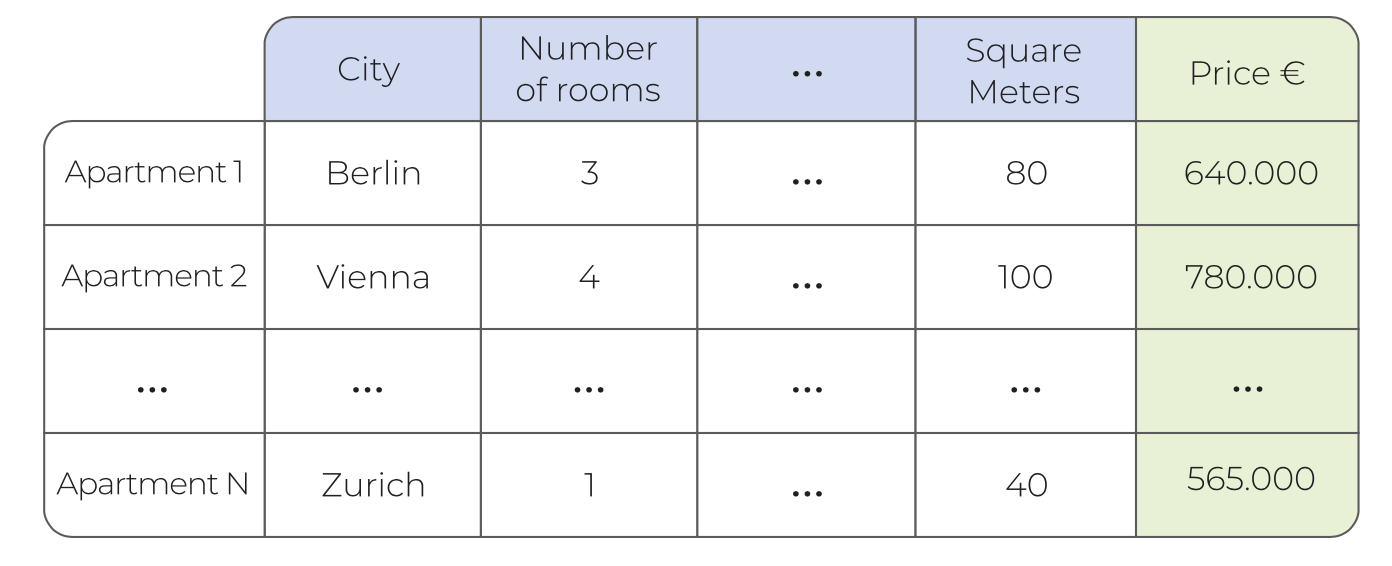
\includegraphics{img/tab1.png}

\hypertarget{variable-de-resultado}{%
\subsection{Variable de resultado}\label{variable-de-resultado}}

La variable de resultado es un solo valor/columna que queremos predecir. A menudo se la denomina \emph{objetivo}, \emph{respuesta}, \emph{variable dependiente} o simplemente denominada \emph{etiqueta}. Como ejemplo, podría pensar nuevamente en el precio de un apartamento:

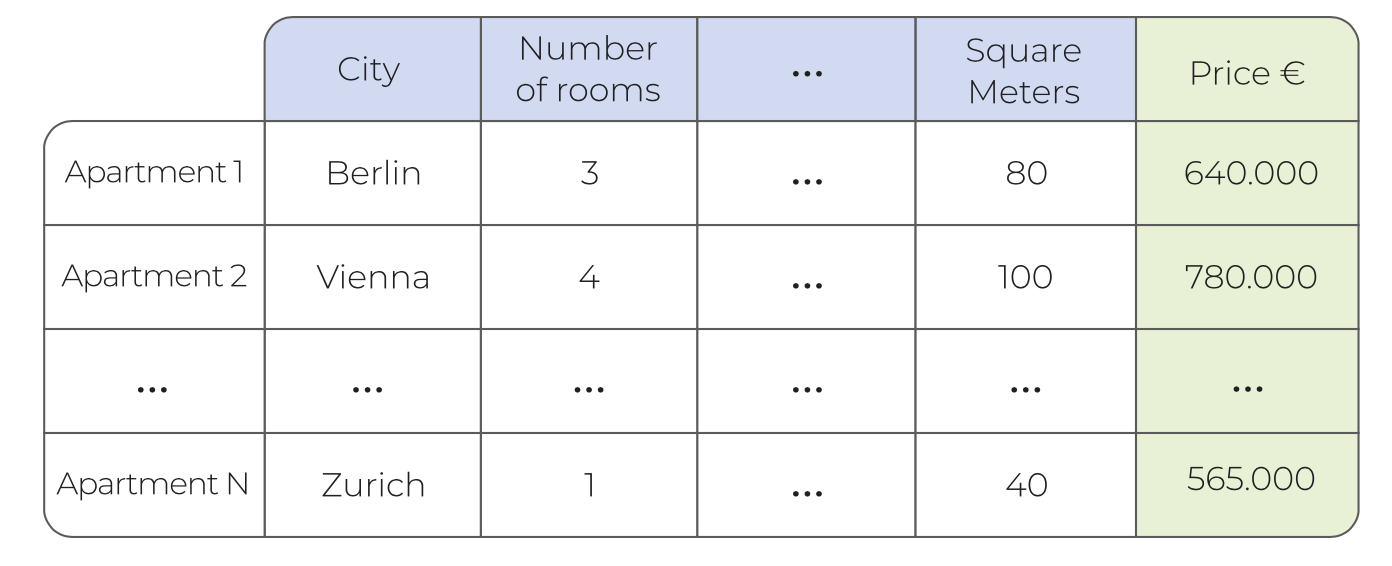
\includegraphics{img/tab1.png}

\hypertarget{regresiuxf3n-vs.-clasificaciuxf3n}{%
\subsection{Regresión vs.~clasificación}\label{regresiuxf3n-vs.-clasificaciuxf3n}}

Dentro del dominio de aprendizaje supervisado, diferenciamos entre modelos de \textbf{regresión} y de \textbf{clasificación}. El modelo específico con el que estamos tratando depende del tipo de datos de la variable de resultado. Si la variable a predecir es continua (como \texttt{numérica}), hablamos de un modelo de regresión. Si la variable es un \texttt{factor} categórico tenemos un problema de clasificación.

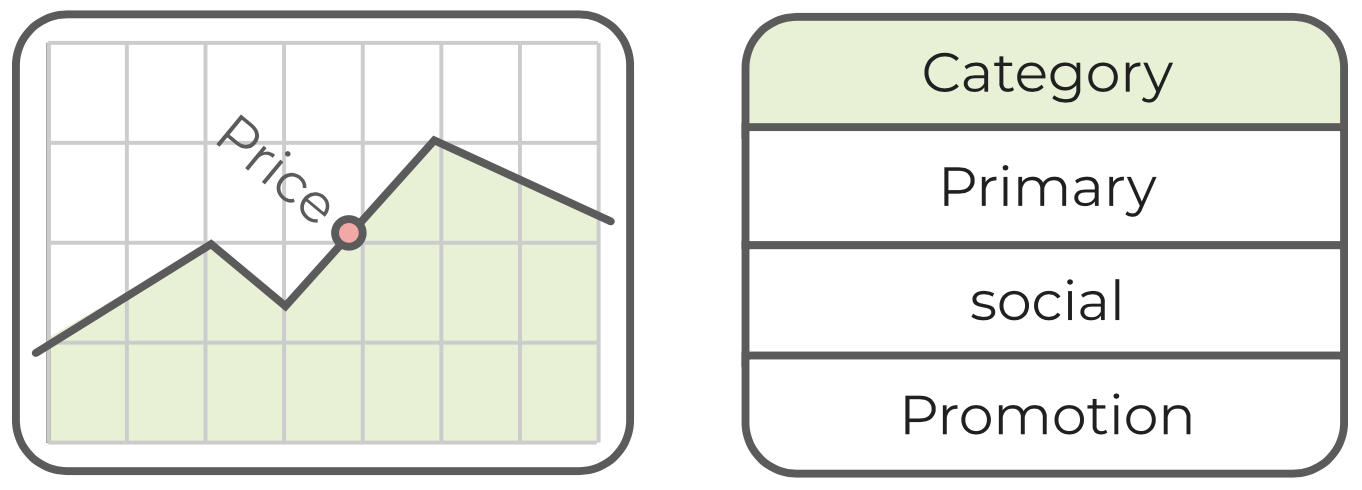
\includegraphics{img/reg.png}

\hypertarget{ejemplo-de-regresiuxf3n-vs.-clasificaciuxf3n}{%
\subsubsection{Ejemplo de regresión vs.~clasificación}\label{ejemplo-de-regresiuxf3n-vs.-clasificaciuxf3n}}

Cuando queremos predecir el precio de un apartamento, la salida es un valor \texttt{numérico} (continuo), lo que significa que estamos tratando con un modelo de regresión. Por otro lado, cuando el cliente de correo electrónico clasifica un correo electrónico en \emph{Primario}, \emph{Social} o \emph{Promociones}, el resultado es un \texttt{factor} (categórico) y necesitamos usar un modelo de clasificación.

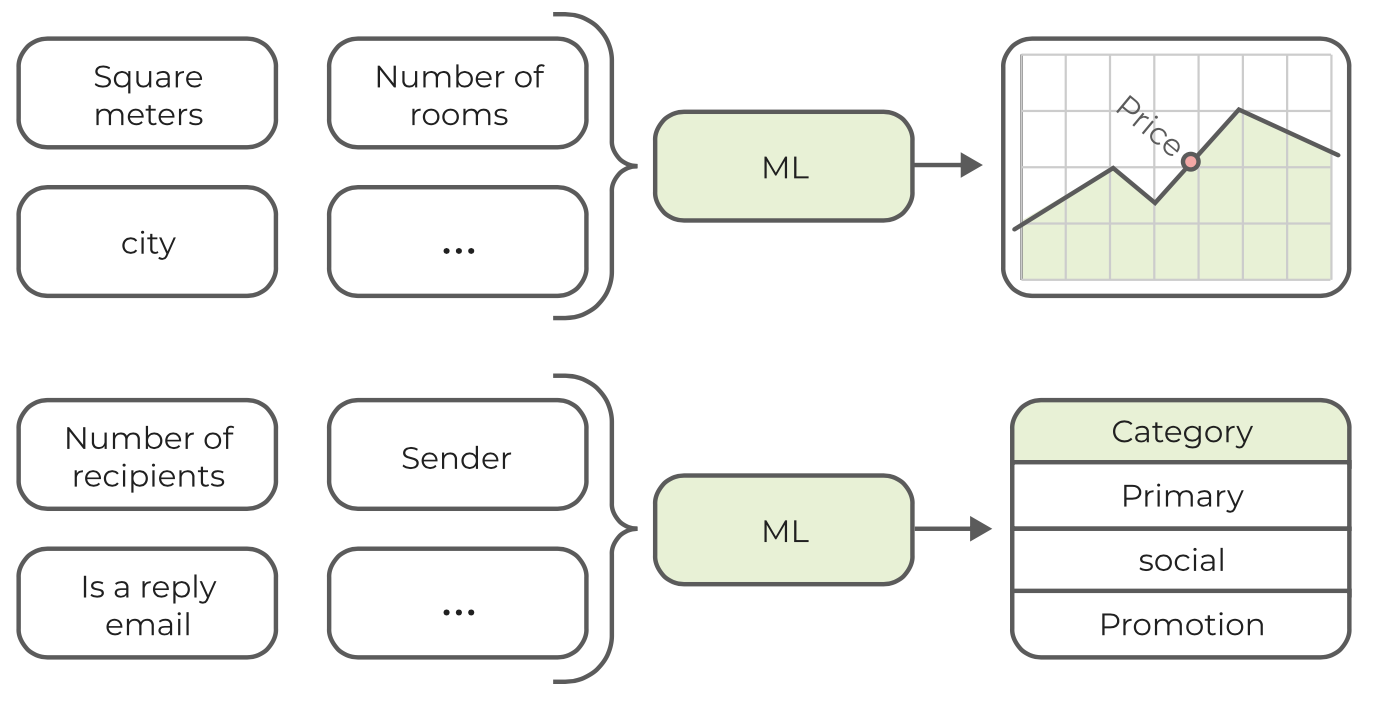
\includegraphics{img/RCE.png}

Todo el material descrito se encuentra en idioma ingles en la página oficial de Quantargo \citep{quantargo2}

\hypertarget{final-words}{%
\chapter{Final Words}\label{final-words}}

We have finished a nice book.

  \bibliography{book.bib,packages.bib}

\end{document}
